\documentclass[a4paper,singleside,12pt]{report} % Uncomment this for single side pdf.
%\documentclass[a4paper,twoside,12pt]{report} % Uncomment this for printing.

\usepackage{ai_bo_thesis}
\usepackage[english]{babel}
\usepackage[T1]{fontenc}
\usepackage{lmodern}
\usepackage{multirow}
\usepackage{graphicx}
\usepackage{subcaption}
\usepackage[section]{placeins}
\usepackage{fixltx2e}
\usepackage{hyperref}
\usepackage{amsmath}
\usepackage[strings]{underscore}


\usepackage[backend=biber,style=trad-plain, sorting=nty,firstinits=true]{biblatex}
\addbibresource{biblio.bib}

\setmainfont{Times New Roman}
\begin{document}
	
	\title{A study of Machine Learning Techniques for Multi-Floor Indoor Localization using Wifi Fingerprinting}
	\topic{Machine Learning}
	\candidate{Muhammad Salman Razzaq}
	\supervisor{Prof.~Claudio Sartori}
%	\cosupervisor{& John Doe, PhD.} % One co-supervisor.
%	\cosupervisors{& Dott.~Ing.~Luigi Bianchi\\& Dott~Avv.~Lucia Rossi} % More than one co-supervisor.
	\academicyear{2020-2021}
	\session{2nd}
	
	\frontispiece 
	\dedication{This thesis is dedicated to everyone who dares to break out of his cocoon and takes a leap of faith to strive for knowledge and betterment.}
	\toc
	\figstoc
	\tablestoc
	\begintext
	
	\chapter{Introduction}
	%YOUR THESIS HERE~\cite{wielemaker2012swi,swi}
		
		\section{Summary}\label{section:summary}
			Over the past decade, there has been a wide-scale increase in intelligent electronic devices such as smartphones, smart-watches, and other devices, which created a broad range of new services, including indoor localization. 
			In scientific terms, the process of acquiring the location or position of a user or device in an indoor environment or setting is known as indoor localization or indoor positioning systems (IPS). 
			The efficacy of satellite technologies (radio waves) in complex infrastructures such as multi-story buildings and roofs is limited due to obstructions~\cite{moore2017super}. 
			Indoor localization uses other novel technologies like Bluetooth beacons, WiFi, etc., to incorporate wearable signal sensors, acoustic, optical, radio waves, and behavioral analysis from intelligent devices.
			    
			Indoor localization is an area of research that is extensively investigated, mainly in logistics and industrial settings by the scientific community over the last decade. 
			The universal proliferation of smartphones and wearable smart devices with networking and communication potentials increased curiosity. 
			Tracking such intelligent devices is synonymous with tracking and localization of respective users enabling a wide range of applications and services. 
			Indoor positioning systems have various applications in navigation systems~cite{mulloni2009indoor}, industries, disaster management~\cite{asimakopoulou2011buildings,borrion2012countering,zelenkauskaite2012interconnectedness}, augmented reality~\cite{huey2011augmented}, health sector~\cite{chen2009dynamic, wyffels2014distributed, }, indoor robotics~\cite{sun2014wifi}, surveillance, building management, and other various sectors. 
			It can also positively influence other novel systems such as intelligent buildings~\cite{}, smart cities~\cite{hashem2016role}, smart grids~\cite{siano2014demand}, the Internet of Things (IoT)~\cite{atzori2010internet}, and Machine Type Communication (MTC)~\cite{taleb2012machine}.
			
			Global Positioning System (GPS) does not perform well in complex indoor environments, thus, creating a void filled by WiFi Positioning System (WPS). 
			WiFi is widely used for networking, communication, and internet connectivity in various private, public, and commercial infrastructures such as airports, hospitals, offices, universities, homes, community centers, industries, nursing homes, and many more. 
			This proliferation makes WiFi an ideal candidate for indoor positioning systems. 
			Many techniques are explored to enrich indoor localization using WiFi, and RSSI is commonly used due to its cost-effectiveness and simplicity. 
			The hindrance with using WiFi RSSI data directly with trilateration methodology is highly constrained by multipath propagation, signal interference, free-space loss, reflection, and refraction~\cite{sadowski2018rssi}. 
			
			In common practice, four main methods are used to acquire the estimated position of the user's device using the signal parameters and wireless concepts of WiFi access points in WPS: fingerprinting based, RSSI based, time-of-arrival based, and angle-of-arrival based approaches. 
			Among these, fingerprinting technology provides better reliability and accuracy~\cite{jang2018indoor} hence making it more suitable. 
			Fingerprinting process is made up of two phases. The first is an offline phase in which the intensity of Received Signal Strength (RSSI) values is measured from known Access Points (AP) to create a virtual indoor map stored as a fingerprint database. 
			The second one is an online phase in which the real-time RSSI values are collected from a user to interpolate the ground truth location with the previously stored fingerprinting database~\cite{youssef2005horus} and estimate the user's position using trilateration. 
			
			A recent scientific study~\cite{liu2012push} explored two main factors that hinder the accuracy of using fingerprinting. 
			1)The difference between RSSI values in the offline and online phase due to changes in the external environment. 
			2) Multiple locations with similar signals due to fluctuations in RSSI signals.
			This reasoning indicates that the limitation is because of both the fingerprint database and the computational memory and power required for database creation whenever the external environment changes and information updates.
			
			The novel research in artificial intelligence and machine learning methods extends a way to resolve this fingerprinting issue~\cite{liu2007survey}. 
			The multivariate regression is the closest approach to predicting x and y coordinates of the user's location in the conventional fingerprinting method. 
			On the other hand, classification treats this problem as a discrete one, predicting a grid-based system-defined space section for the user's location. 
			The overall structure should be divided into multiple grids, and the system should label all the grids. 
			In indoor localization with classification, the model will predict the discrete labelled value of location~\cite{belmannoubi2019stacked}. 
			This study highlights the importance of indoor positioning as a grid-based problem. It is essentially applicable for guiding personnel in a complex area and locating patients in the nursing home. 


		\section{Thesis Contribution}

			In this thesis, we explored the scientific process of indoor localization systems in depth. 
			We investigated indoor localization techniques such as RSSI, channel state information, fingerprint analysis, angle of arrival, time of flight, and time difference of arrival. 
			We also examined various technologies such as WiFi, Bluetooth, Zigbee, acoustics, optical, and RFID applied in indoor positioning systems. 
			We also researched real-life applications of IPS in public, private and commercial sectors to signify the importance of this process in the contemporary world.
			
			We studied the requisites of the data features in an indoor positioning system. 
			We examined several datasets publicly available and selected three from them to perform our experiments. 
			The primary dataset is the most widely used public dataset collected in Jaume I University, Spain. 
			This dataset is based on RSSI values collected from 520 WiFi access points, along with information on users' location in three predefined buildings in the university. 
			
			We applied various state of the art machine learning methodologies and techniques to this well-developed UJI Indoor fingerprinting database. We investigated the problem from three perspectives. 
			Initially, we used a grid-based approach to classify the location of the user using predefined labels. 
			In these experiments, we developed a pipeline of feature preprocessing, feature engineering, and machine learning models to predict the user's location in three buildings both separately and as one complete dataset. 
			We used eight different classifiers for model selection and tuned hyperparameters to create a new benchmark against the existing literature. 
			The researchers at the School of Computer Science and Engineering Nanyang Technological University, Singapore benchmarked 86.34\% on the UJI Indoor dataset~\cite{yean2020feature}, whereas our experiments have achieved an accuracy of 88.82\%. 
			
			Moreover, we took the approach of regression to refine the results achieved through the fingerprinting process. 
			We applied principal component analysis and other feature engineering steps to refine our dataset. 
			We developed a multivariate regression model pipeline to predict the latitude and longitude of the user's device. 
			After performing a model selection on over seven regression models, we tuned a K-Nearest Neighbour regression model to achieve an RMSE error of 3.637 meters.
			
			To further investigate the expressiveness of artificial intelligence in this domain, we developed a three-stage cascaded machine learning model to estimate the user's location. 
			The first stage is comprised of a Random Forest classifier to predict the building of the user. The second stage used the output of the first stage to make a local prediction on the floor of the user's position. 
			Finally, a global regression model predicts the coordinates of the user's location. 
			
			The dataset does not contain information about the location of the WiFi access points (WAPs). 
			We studied and applied trilateration to estimate the position of WAPs based on the RSSI signal strength for users. 
			We examined the optimization of access points location for better reach to the audience.    

	\chapter{Literature Review}

		\section{Indoor Localization}
			\subsection{Techniques for Indoor Localization}
				In this section, we shall discuss various techniques that we can employ in the field of indoor localization~\cite{zafari2019survey}. In general, we have three types of localization:
				
					\begin{itemize}
				
					\item  \textbf{Device-based localization (DBL):}  In this process, a user device estimates its relative position concerning some Reference Nodes (RN). Its main application is in navigation, where it assists users in locating itself around indoor and outdoor spaces
					\item  \textbf{Monitor based localization (MBL):} In this process, a set of reference nodes acquires the user's or devices` location connected to the anchor node passively. This process, generally, remains in continuous operation and is mainly used for tracking purposes to apply various applications.
					\item  \textbf{Proximity Detection:} This methodology refers to proximate the distance between a Point of Interest (PoI) and the user's location. This type is mainly used in context-aware services where it provides cost-effective and reliable operations. 
				
					\end{itemize}

				\subsubsection{Received Signal Strength Indicator (RSSI)}
					The received signal strength is the actual strength of the signal that is perceived by the receiver. 
					It is usually measured in milliWatts (mW) or decibel-milliwatts (dBm).  
					The value of RSS varies inversely with the distance between a receiver device and a transmitter (Tx).  
					It is usually measured on a negative scale, so the higher the value of RSS, the less will be the distance between the source and the receiver. 
					This technique is one of the simplest and universally used techniques for indoor positioning systems~\cite{ladd2005robotics, krishnan2004system, haeberlen2004practical, castro2001probabilistic, yang2013rssi}.
					
					Once the absolute position of one of the two devices is known, we can estimate the distance between them using various signal propagation techniques. 
					RSSI, which differs from RSS, is just the indicator for signal strength with arbitrary units. 
					For example, Cisco defines its range in between 0 and 100, whereas Atheros WiFi chipset uses a range of 0-60 to determine its RSSI values. 
					Although RSSI based indoor localization is cost-efficient and straightforward, it is prone to poor localization accuracy, particularly when there is no clear Line of Sight as walls and other significant obstructions cause fluctuation in RSS signals because of additional multipath interference and fading.~\cite{xiao2013pilot,yang2013rssi}
					
					In the device-based localization (DBL) process, the RSS-based technique requires an application of trilateration methodology. 
					In the pure trilateration procedure, we use the location of at least three devices and the signal strength from these devices to the signal user device. 
					We apply the geometric and trigonometric formulas on the three spheres created by the propagating signal to find the absolute distance between the user's device and the sources, as depicted in figure~\ref{fig2.1}. 
					In monitoring-based localization, a similar process is used, and the user's information is continuously monitored and transmitted to a server-based data storage device for further applications. 
					However, in the case of proximity-based localization, we create geofencing using only one device and detect whenever the user's device enters the signal propagation sphere of our source. 
					We can use this application for marketing purposes where we, a retailer or a franchisee, detect whenever a user enters its outlet to target its marketing alerts more purposefully. 
					
					\begin{figure}[!htb]
					\centerline{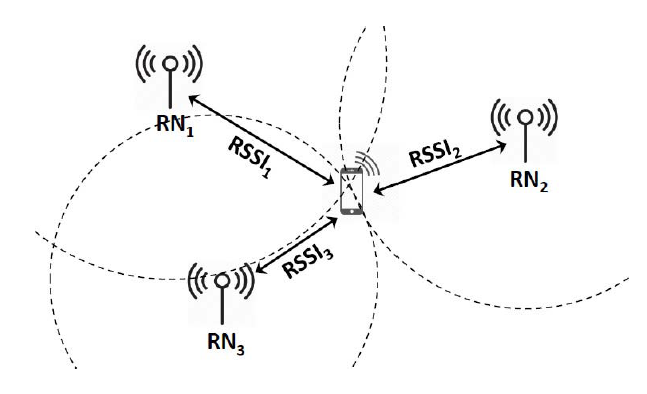
\includegraphics[width=0.8\textwidth]{./figures/RSSI-indoor-localization.png}}
					\caption{User device localization based on RSSI}
					\label{fig2.1}
					\end{figure}

				\subsubsection{Channel State Information (CSI)}
					In wireless signal propagation, phase behaviour and amplitude vary for different frequencies. 
					The signal's bandwidth that makes the wireless channel frequency-selective is usually greater than the channel's coherence bandwidth in UWB, IEEE802.11 and other wireless systems. 
					Furthermore, based on the signal's wavelength and antennae distance, there exists a significant variation in channel frequency responses in multiple antennae transceivers. 
					RSS only provides us an approximation of the average amplitude over the accumulated signal overall antennae and the entire signal's bandwidth. 
					Although RSS is generally used because of its minimal hardware requirements and simplicity, this phenomenon makes it prone to interference and high variability. 
					On the other hand, Channel Frequency Response (CSR) considers the amplitude and phase responses of the signal between separate receiver-transmitter pairs of antennae. 
					CSR captures responses for various signal frequencies, making its resolution more granular and leading to better accuracy.  

				\subsubsection{Fingerprint Analysis}
					This analysis constitutes creating a virtual map by performing an environmental survey to acquire features or fingerprints of the target location. 
					This process is also called scene analysis as we recreate the environment where our localization system will be installed. 
					It consists of an offline phase for collecting the fingerprints and creating a virtual map and an online phase where we predict the user's location in real-time~\cite{youssef2005horus, zafari2015microlocation}. 
					Both RSSI and CSI methods are used to capture the fingerprints in this process. 

					As explained above, this methodology utilizes the offline phase to develop a grid-based virtual map where each grid can be associated with specific values of the RSSI or CSI signal strengths. 
					After this creation, we can deploy various probabilistic and artificial intelligence-based techniques to estimate the user's location based on the virtual map created before. 
					All the grids are associated with specific RSSI or CSI values; this method provides a discrete estimation of the user rather than the continuous one. 
					Therefore, the granularity and resolution of our approach depending upon the size of these grids. 
					
					In theory, if we increase the grid density by reducing the distance between grids, the granularity of the user's location estimation should increase to the extent that we can make it continuous. 
					However, this can only be achieved to a limit as reducing the size between grids would induce more noise and interference between the signals in the nearby grid, hence sabotaging the accuracy of the prediction in a specific grid. 
					This effect would also depend upon the type of signal used as RSSI's would be much more prone to this effect than CSI as the difference in the signal strength between neighbouring cells diminishes. 
					This phenomenon marks an essential trade-off between the probability of correct location prediction and the granularity of the fingerprinting position that must be considered while choosing the parameters and location for this localization process. 
					It is noteworthy to mention that as this process includes an offline and online phase, it is highly prone to change in the structure of the location over time. 
					Whenever there is a change in design or the signal transmitters on the site, we would have to repeat the whole process of developing fingerprints.   

				\subsubsection{Angle of Arrival (AoA)} 
					One of the distinguishing features of signal theory is that we can use its various components in real-life applications. 
					In our use case of indoor localization, we can estimate the user device's location by calculation the angle at which it receives the signal from the estimator. 
					This approach requires antennae arrays~\cite{xiong2013arraytrack} on the receiver end to estimate the signal angle at which the receiver receives the signals from known transmitters. 
					We also consider the time difference at which the different antennae in the array receive the signal.
					Figure~\ref{fig2.2} illustrates the angle of arrival that we can use to estimate the user's location. 
					
					\begin{figure}[!htb]
					\centerline{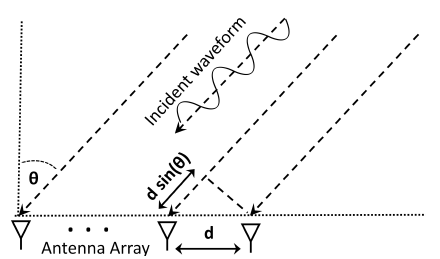
\includegraphics[width=0.8\textwidth]{./figures/AoA-indoor-localization.png}}
					\caption{User device localization with AoA}
					\label{fig2.2}
					\end{figure}
					
					AoA is more accurate than RSS techniques, but it requires more sophisticated hardware with complex and careful calibrations. 
					This approach works best when the distance between transmitter and receiver is small. 
					It is prone to high error~\cite{kumar2014accurate} as this distance increases because a small error in angle calculation amplifies into a big error in location estimation. 
					Furthermore, various effects in indoor environments deteriorate the angle of arrival in terms of the line of sight, so it is better used for small distances in outdoor environments. 

				\subsubsection{Time of Flight (ToF)}

					Like Angle of Arrival, Time of Flight (ToF) estimates the distance between the receiver and transmitter~\cite{dargie2010fundamentals} using the signal propagation time. 
					It is also known as the Time of Arrival. 
					As we know, that the electromagnetic signal propagates with the speed of light, so by taking the product of the constant of light $c = 3 x 10^8 m/sec$ by the time difference in between propagation of a signal from the transmitter and the time at which it reached the receiver, we can estimate the distance between them. 
					
					\begin{figure}[!htb]
					\centerline{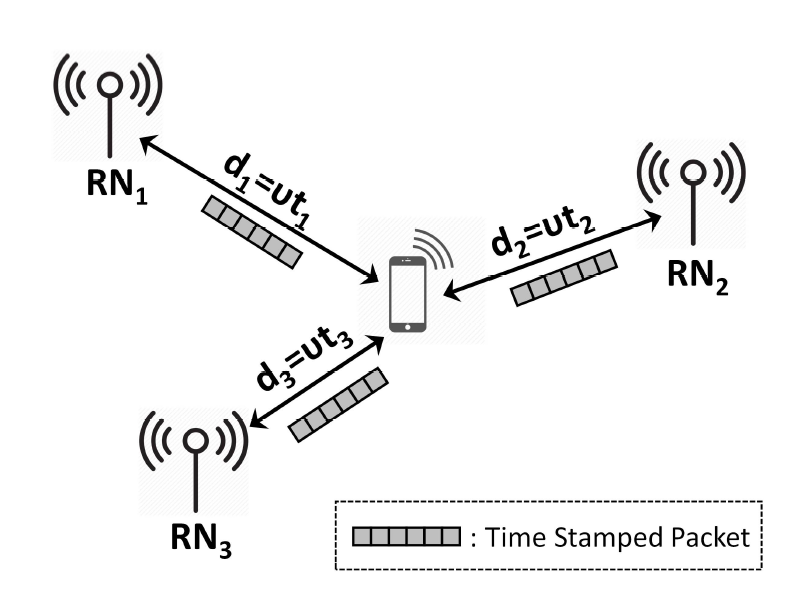
\includegraphics[width=0.8\textwidth]{./figures/ToF-indoor-localization.png}}
					\caption{User device localization with ToF}
					\label{fig2.3}
					\end{figure}
					
					As similar to received signal strength (RSS), this phenomenon can also be used in distance-based and monitor-based localizations. 
					In figure~\ref{fig2.3}, we can see time-stamped packets from three different sources can help localize the user's device. 
					Here, similar to trilateration, basic geometry can be used to estimate the user's position. 
					Sampling rate and signal bandwidth directly influence the accuracy of this process. 
					Moreover, ToF requires transmitters, receivers and time-stamped data packets to be synchronized concerning the transmission protocol used. 

				\subsubsection{Time Difference of Arrival (TDoA)}
					This process is different from ToA because it utilizes the difference measured in signal propagation times on reception from varied transmitters. 
					The ToF uses the absolute time of signal propagation, whereas this process creates a hyperboloid for various transmitters by converting the time difference to physical distance, as shown in figure~\ref{fig2.4}. 
					We can estimate the user's location by determining the resultant of these hyperboloids~\cite{liu2007survey}. 
					Here, again, at least three transmitters are required to calculate the user's location.

					\begin{figure}[!htb]
					\centerline{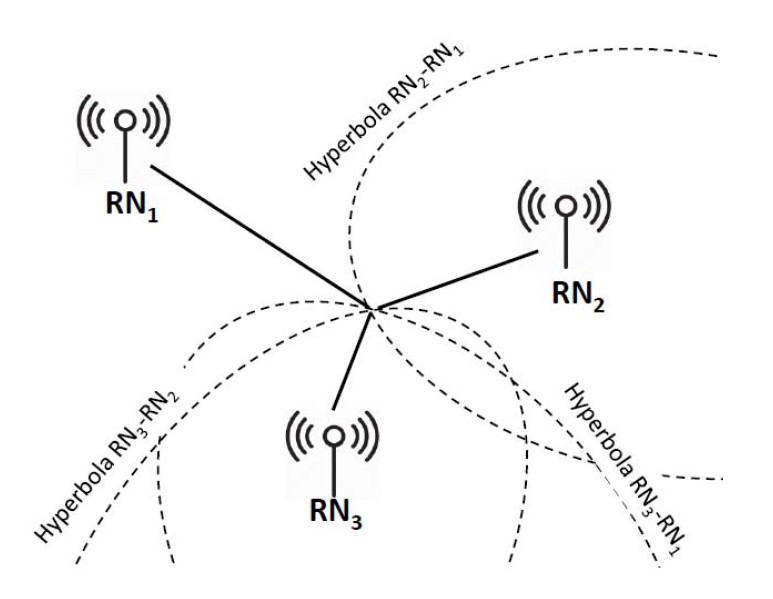
\includegraphics[width=0.8\textwidth]{./figures/TDoA-indoor-localization.png}}
					\caption{User device localization with TDoA}
					\label{fig2.4}
					\end{figure}
					
					The presence of a direct Line of Sight (LoS) directly affects the performance of TDoA. 
					It also depends upon the signal sampling rate at the received and signal's bandwidth. 
					In TDoA, there is the necessity of synchronization between the transmitters, whereas, in ToA, synchronization is required between the receiver and the transmitter.


			\subsection{Technologies for Indoor localization}


				Various existing technologies applied for indoor localization will be discussed in this section. 
				We will elaborate on radio communication technologies like WiFi, ZigBee, Bluetooth, and RFID. 
				We would also take into account several new emerging acoustic and light-based technologies. 
				Although computer vision can also be used for this purpose, this is beyond the scope of the thesis, so it would not be discussed here. 
				
				\subsubsection{WiFi}

					The majority of the current laptops, smart-phones, smart-watches, and other portable user devices use WiFi for internet connectivity.  
					WiFi operates typically in the Industrial, Scientific, and Medical (ISM) band, based on IEEE 802.11 standard. Its primary use is networking and internet connectivity for various electronic user devices in commercial, public, corporate, and private environments.  
					
					Initially, the range for regular operations of WiFi was about 100 meters~\cite{liu2007survey}, but with the advancement in technology, its capacity and range have increased to about 1 kilometer~\cite{centenaro2016long,adame2014ieee} in IEEE 802.11ah standard, which is mainly used for IoT purposes. 
					WiFi is an ideal contender for indoor positioning systems and is one of the most widely researched technology in the scientific literature~\cite{vasisht2016decimeter,kumar2014accurate,xiong2013arraytrack,kotaru2015spotfi,xiao2013pilot,paul2009rssi,jiang2012ariel,woo2011application,chintalapudi2010indoor,liu2012push,liu2011wifi,feng2011received,cypriani2009open,zou2014online,ciurana2007wlan,hoang2013parameter,kang2012improved}. 
					As the existing infrastructure of WiFi access points already has several Reference Nodes (RN), we can use it for basic localization systems with good accuracy without additional hardware installation~\cite{kumar2014accurate}. 
					
					We should consider that the primary purpose of WiFi technology is for data transfer, networking, and communication. 
					It is not optimized for localization; therefore, artificial intelligence and other novel algorithms should be incorporated on top of the technology to achieve high accuracy. 
					WiFi is also prone to uncontrolled signal interference as it operates in the ISM band, hence deteriorating its accuracy.  
					WiFi can use various techniques discussed in the previous section, such as CSI, RSSI, AoA, ToF, and their hybrid combinations for its application in positioning systems.

				\subsubsection{Bluetooth}

					IEEE 802.15.1 standard, commonly known as Bluetooth, refers to a technology primarily used in personal spaces to connect different moving or fixed devices. 
					It comprised of the physical and MAC layers specification and worked in the range of 20 meters initially. 
					Recent improvements in the technology have led to a new version~\cite{zafari2015microlocation}, Bluetooth Low Energy (BLE), that has an improved range of 70-100 meters and a better capacity of 24 Mbps for data transfer. 
					
					BLE, generally known as Bluetooth Smart, can be integrated with various aforementioned techniques like RSSI, ToF, and AoA for localization. 
					However, RSSI is mainly used in BLE due to its simplicity and sophistication. RSSI, due to its proneness to various interference effects, limits the accuracy for BLE localization systems. 
					Although BLE in its original form has applications for localization, two BLE-based protocols Eddystone and iBeacons, have been proposed by Google Inc. and Apple Inc., respectively. 
					
					IBeacons protocol is mainly designed for proximity-based services. 
					In 2013, Apple announced this product at the World Wide Developer Conference (WWDC)~\cite{apple-ibeacon}. BLE-enabled devices use this protocol to transmit periodic low-energy signals. 
					The principal operation of this technology is illustrated in figure~\ref{fig2.5}, where UUID refers to the Universally Unique Identifier (UUID) of the device. 
					Any BLE enabled the device in its proximity to pick up these signals or beacons and uses RSSI to estimate the proximity between the user and the iBeacon. 
					
					\begin{figure}[!htb]
					\centerline{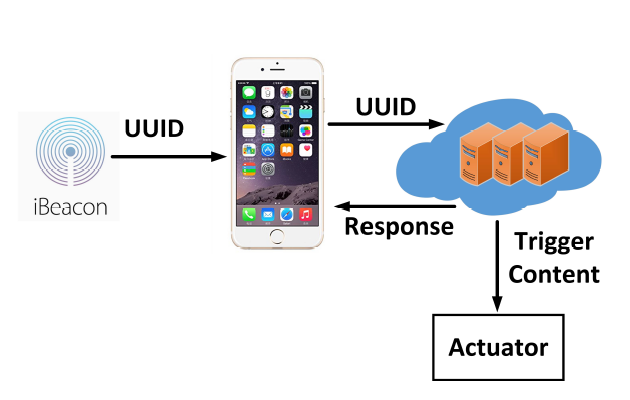
\includegraphics[width=0.8\textwidth]{./figures/iBeacon-indoor-localization.png}}
					\caption{iBeacon operational architecture}
					\label{fig2.5}
					\end{figure}
					
				\subsubsection{ZigBee}

					IEEE 802.15.4 standard developed with the MAC and physical layers for low data rate, cost-effectiveness, and energy-efficient personal area networks lay the foundation of ZigBee technology~\cite{baronti2007wireless}. 
					Zigbee is primarily used in wireless sensor networks with higher levels of the protocol stack. Zigbee consists of a layer and an application layer. 
					The application layer is responsible for developing applications and communication distribution, whereas the networking layer deals with network organization and multihop routing. 
					Zigbee is still not readily available on most portable networking devices; therefore, it is not appropriate for indoor localization.

				\subsubsection{Radio Frequency Identification Device (RFID)}

					This technology mainly works on electromagnetic transmission from a transmitter to any Radio Frequency (RF) enabled circuit~\cite{holm2009hybrid}. 
					Its primary purpose is the storage and transmission of data. RFID systems consist of a tag and a reader, which communicate with each other. 
					A predefined RF and protocol enable RFID readers to read data emitted from RFID tags. There are two types of RFID systems.
					
					\begin{itemize}
					
					\item  \textbf{Passive RFID:} This type can work without batteries but has a limited communication range (1-2m). They can work in low, high, microwave, and UHF frequency ranges and are generally cheaper, smaller, and lighter than active RFIDs. They can work in place of bar codes, especially when concealed, as they do not require Line of Sight (LoS) to operate. However, they are not good candidates for indoor localization due to their minimal range.
					\item  \textbf{Active RFID:} They operate in microwave and UHF (ultra-high frequency) range. They require batteries or a power source to operate. They can transmit their ID periodically over a range of hundreds of meters from the RFID reader. They have low cost, good range, and flexibility to be embedded in tracking objects, making them a suitable candidate for indoor localization. This technology still has not achieved very high accuracy, limiting its use primarily to proximity-based devices. 
					
					\end{itemize}


				\subsubsection{Visible Light}

					The technology that uses visible light between 400-800 THz modulated and emitted mainly by Light Emitting Diodes (LEDs) is known as visible light communication (VLC). 
					Localization techniques based on VLC primarily use light sensors to estimate the direction and position of the LED emitters. 
					This technology is an emerging technology for high speed data transfer~\cite{kuo2014luxapose}, and its use for localization in the commercial sector has increased over the past few years. 
					
					Visible light communication used LEDs similar to iBeacons to transmit the signals that the sensor/receiver detects for localization. 
					The Angle of Arrival (AoA) is considered as the most accurate localization technique~\cite{kuo2014luxapose,armstrong2013visible} for this technology. 
					The main advantage for VLC based localization is scalability which is even greater than WiFi. 
					Nevertheless, a fundamental limitation is that light travels in straight lines; hence constraints in the Line of Sight (LoS) between the sensor and LED lead to inaccurate localization.  

				\subsubsection{Acoustic Signal}
					In this technology, the receiver nodes act as sound sources emitting acoustic signals detected by a microphone in intelligent devices to proximate the user`s location concerning the source. 
					Acoustic signals primarily use the Time of Flight (ToF) technique for localization~\cite{liu2013guoguo}. The acoustic signal that the source emits contains timestamps which enable microphone sensors to localize themselves. 
					This technology also enables us to estimate the velocity~\cite{huang2014swadloon} and relative position of the user`s device by detecting frequency and phase shifts in received signals using Doppler effects.
					
					This technology has a significant concern of noise pollution as smart-phone microphone limitations such as anti-aliasing filter, and sampling rate limits the high accuracy for only audible band acoustic signals (<20KHZ). 
					Therefore, for the appropriate application, the transmission power should be low enough to be perceivable by the human ear, and it should be improved at the receiver`s end using advanced signal processing algorithms. 
					Furthermore, the need for a high update rate impacting the device`s battery and additional infrastructure of source nodes make acoustic signal not a suitable candidate for localization.  

			\subsection{Applications of Indoor Localization}


Indoor localization provides us information about the position of objects and personnel in indoor environments. In this section, we would look into the real-life implemented application of indoor localization.

				\subsubsection{Factories}

					In factories, indoor localization can be used in various ways to locate machines, objects, goods, vehicles, and employees. 
					We can quantify some of the applications of indoor positioning systems in industries.

				\textbf{Asset Tracking:} 
				Object and asset tracking is essential to industries and logistics in cost-effectiveness, theft protection, time savings, lean management, and process optimization. 
				With the help of the localization of goods and vehicles, we can also use external sensors and actuators to control various environmental factors in industry such as humidity, pressure, and temperature. 

				A usual warehouse contains thousands of goods waiting to be delivered or processed. It is essential to locate them in time for the smooth functioning of the supply chain. 
				Integrated digital display with indoor localization solutions could help locate these goods and provide necessary instructions to the workforce. 
				In addition to goods, pallet trucks, forklifts, and tugger trains can also be tracked, ensuring lean and optimized process management.
								
				 \textbf{Localization of Employees:}
				Efficient workflow management and process optimization can be achieved through integrated tracking of employees on site. 
				In addition, this process could also ensure the security and safety of employees and assets. 

				With the advancement of technology, working conditions in industries have become critically hazardous. 
				Process safety management principles allow only trained employees to work in danger zones that this process could be ensured. 
				On top of the day-to-day operations, geo-based localization can assist in emergencies like a fire, chemical spill out, etc. It is necessary to evacuate users to the assembly points in case an emergency breaks out. 
				This solution can be integrated into the name tags and ensure the safety of employees.
 
				Moreover, we can monitor environmental conditions like temperature, air quality, humidity, and light to ensure safe and healthy working conditions for the users. 
				This technology can also ensure industries` compliance with ISO 45000 (occupational health and safety) and ISO 14000 (environmental management systems).
				
				\subsubsection{Airports and Railway Stations}

					Indoor positioning systems (IPS) can ensure smooth and painless travel by assisting passengers, employees, airways, railway companies, and associated businesses. 
					IPS can provide indoor navigation, real-time asset tracking, tracking solutions and analyses, parking management. 
					It can increase the overall comfort and efficiency of travelling solutions.
					
					In terms of user, IPS can be used as a way-finder to find a way through complex airports and railway infrastructure to reach their desired gate. 
					It can also provide information about available food and shopping options in complex arenas. 
					It can also assist users with parking management and reducing waiting time through optimization of queue management. 
					
					For airport authorities and retailers, IPS can revolutionize their work efficiency and revenue generation.
					IPS can allow companies to send targeted discount coupons and advertisements to users based on their interests and location. 
					Airport authorities can optimize security guards' location, staff, passenger and inventory management, track expensive goods, and airport employees to assign geo-based tasks, hence, improving the efficiency of the workflow. 
					Moreover, this collected data can be used for real-time monitoring of passenger flow and data analytics for schedule management and process optimization. 

				\subsubsection{Market Research}

					In recent years, digital marketing has shaped up merchandising by companies. 
					Neuroscience knowledge and tools are used to study the behavior of consumers using the data collected through various digital applications. 
					This scientific field is known as neuromarketing, which also involves processing information, determining users' meaning and emotional value, and then applying analysis on the findings to target advertisements. 
					
					IPS can track users' location in various sections of the shopping malls to analyze customers' paths and time of stay. 
					This information can be integrated with various neuromarketing techniques~\cite{fortunato2014review} like EEG~\cite{yadava2017analysis}, BVP~\cite{rosenlacher2020effect}, eye tracking~\cite{ungureanu2017neuromarketing}, and GSR~\cite{cuesta2018case}. 
					This integration can register the users' emotions while passing throughout the route, which can help retailers send improve their products, optimize floor plans, and target marketing campaigns.

				\subsubsection{Supermarkets and Shops}

					Indoor localization can improve the shopping experience of users in extensive and complex supermarkets. 
					They can assist users to navigate through sections of the mart and go to their desired products. 
					They can also help locate the discounted products. 
					It can also help users in selecting those outlets for shopping that satisfy all their shopping need cost-efficiently.
					
					IPS can assist retailers in stock, asset, and inventory management. 
					They can use IPS and market basket analysis to optimize the floor, and product placement plans to increase sales and revenues. 
					RFID-based IPS can also improve the security situation of supermarkets by ensuring theft control.

				\subsubsection{Hospitals and Nursing Homes}

					In line with the aforementioned applications, IPS can be used in nursing homes and hospitals to navigate patients and employees.
					It is also valuable for processes, goods, and tools management. 
					They can be critical in improving the workflow in hospitals and old care homes as they could locate emergencies to doctors and health care workers. 
					Patients who have dementia, Alzheimer's disease, and other neurological disorders can stray in complex buildings. 
					They can be located and provided with the necessary help with IPS. 
					Furthermore, the equipment in hospitals is costly with limited supply mostly, so it is necessary to locate them for protection and necessary use optimization. 


	\chapter{DataSet}
		\section{UjiIndoor Loc Dataset}~\cite{ujiindoor-data}
			\subsection{Description of elements stored}

				\subsubsection{1) RSSI Levels}

					The WAPs identified and their RSSI level values are the utmost essential knowledge for WLAN fingerprinting differentiation. 
					This information constitutes 98\% of the statistics in every record, which is 520 vector positions out of 529, denoting 520 element vectors of integers in the dataset. 
					These statistics denote the RSSI levels, while WAP identifiers are associated with vector positions. 
					Presentation in this way has been acquired due to the numerous contrasting WAPs identified in the three buildings, i.e., 520 and Android application, which gives RSSI levels in integer numbers.
					
					The technique getScanResults()~\cite{android-wifi-manager} which is a part of WifiManager~\cite{android-wifi-getscan-method} of Android class, is adopted to acquire records for identified WAPs for all the devices. 
					The MAC addresses are encrypted as strings, and the RSSI levels coincide with negative values taken in dBm, while 0dBM denotes that the identified WAP`s signal has an excellent strength and as the value decreases, the strength of the signals weakens. 
					The 520 WAPs have their associated MAC addresses, which are a part of the database. 
					These MAC addresses have been arranged alphabetically and retitled to $WAP_{nnnn}$ in an orderly manner. 
					These new identifiers are acknowledged as a replacement to MAC addressed for data privacy and governance. 
					
					The database contains a sum of 520 WAPs. 
					The 520-dimensional vector for each observation has the primary intensity RSSI magnitude from the identified WAPs in one wifi screening; all WAPs are not identified in one screening. e.g., one of the scans detected only 14 WAP identifiers. 
					The detected WAPs RSSI levels stay unchanged, and the database uses the artificial value +100dBm by default for the particular WAPs that the device could not identify.

				\subsubsection{2) Real-world coordinates}

					There are three features in every observation (521 to 523 vector position) by which the real world coordinates are depicted; the floor of the building and the longitude and latitude coordinates (in meters with UTM from WGS84~\cite{janssen2009understanding})

				\subsubsection{3) Space identifiers}

					BuildingID denoted by vector position 524 is represented by integers (0-2); this correlates with the building in which the observation was taken. 
					The three buildings of the School of Technology and Experimental Sciences (center image) of UJI University campus (left); hereafter ESTCE; and zoom inside the third floor of the TI building (right) has been shown in figure~\ref{fig3.1}. 
					Table~\ref{table3.1} exhibits the BuildingID associated with each building of the ESTCE.

				
					\begin{table}[!htb]
					\centering
					\begin{tabular}{ll}
					\hline
					Real Building & Building ID \\ \hline
					ESTCE - TI           &0    \\
					ESTCE - TD          &1    \\
					ESTCE - TC          &2    \\ \hline
					\end{tabular}
					\caption{Relation between real building and BuildingID.}
					\label{table3.1}
					\end{table}
					
					\begin{figure}[!htb]
					\centerline{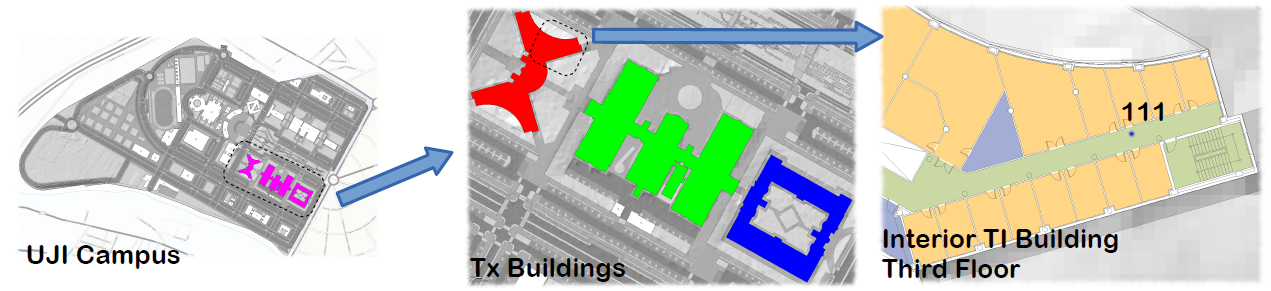
\includegraphics[width=1.2\textwidth]{./figures/map_of_buildings.png}}
					\caption[Map of the UJI Riu Sec Campus and zoom on the Tx Buildings.]{  Pink refers to the ESTCE - Tx building on the UJI Campus map (left). On the Tx building zoom (right): red refers to TI building, green corresponds to TD building and blue stands for TC building. On the interior of TI building, the blue point is the reference point.}
					\label{fig3.1}
					\end{figure}

					The $525^{th}$ position of a vector that is a representation of every reading is named as spaceID. 
					It has one integer value, which for any particular example is taken to detect the specific space where the capture was observed; this could be an office, a lab, etc. 
					The $526^{th}$ place provides its location corresponding to the spaceID. It represents the inside (value 1) or outside (value 2) space where the user captured the reading. 
					Outside denotes the space in front of the door in the corridor. As an illustration, the calculations on the $7754^{th}$ data point of these fields are manifested in table~\ref{table3.2}. 
					As per this table, the capture was taken in a reference space located outside office 111 at ESTCE -TI building (TI).
					
					\begin{table}[!htb]
					\centering
					\begin{tabular}{llll}
					\hline
					Floor & BuildingID & SpaceID & Rel.Pos. \\ \hline
					3     & 0          & 1111    & 2   \\     \hline 
					\end{tabular}
					\caption{Reference point where the $7754^{th}$ record was taken.}
					\label{table3.2}
					\end{table}
				
					There are two database variants; one is called the training subset, and the other is the validation subset. The training subset has properly defined reference points that at least two different users caught. 
					The values are taken randomly; just like the real-time localization system, the point of reference (determined by space ID and relative position) are not placed in the validation records. 
					This information is represented by the number 0 for these two fields in the validation dataset. 

				\subsubsection{4) User Identifier}

					The $527^{th}$ dimension of vector places userID as integer numbers from 1 to 18. 
					These digits represent eighteen users who took part in the procedure and produced the training subset. 
					This field is not recorded in the validation dataset, so 0 represents it. Every individual’s height is also given~\cite{ujiindoor-data}. 
					This identifier is helpful because of the effect the spatial site has on the calculated RSSI measurements~\cite{1331706}. 




				\subsubsection{5) Phone Identifier}


					In the same manner (location 528) has an integer value representing Android phones used in the process. 
					Table~ref{table3.3} exhibits the correspondence between every PhoneID and its corresponding device (model and version). 
					Aforesaid users from USER0001 to USER0018 took part in the generation of the training set. 
					However, USER0000 represents that the phone is utilized to create the validation dataset. Total twenty phones are used (twenty-five in the case of the Android version). 
					In some instances, few users have similar smartphone models. Nexus 4, in particular, is used by three different users. 
					They also took part in developing the validation dataset. Similarly, an LT22i mobile set is used by two different users to create training samples. 

				\begin{table}[!htb]
				\centering
				\begin{tabular}{llll}
				\hline
				PhoneID & Android Device     & Android Ver. & UserID   \\ \hline
				0       & Celkon A27         & 4.0.4(6577)  & 0        \\
				1       & GT-I8160           & 2.3.6        & 8        \\
				2       & GT-I8160           & 4.1.2        & 0        \\
				3       & GT-I9100           & 4.0.4        & 5        \\
				4       & GT-I9300           & 4.1.2        & 0        \\
				5       & GT-I9505           & 4.2.2        & 0        \\
				6       & GT-S5360           & 2.3.6        & 7        \\
				7       & GT-S6500           & 2.3.6        & 14       \\
				8       & Galaxy Nexus       & 4.2.2        & 10       \\
				9       & Galaxy Nexus       & 4.3          & 0        \\
				10      & HTC Desire HD      & 2.3.5        & 18       \\
				11      & HTC One            & 4.1.2        & 15       \\
				12      & HTC One            & 4.2.2        & 0        \\
				13      & HTC Wildfire S     & 2.3.5        & 0,11     \\
				14      & LT22i              & 4.0.4        & 0,1,9,16 \\
				15      & LT22i              & 4.1.2        & 0        \\
				16      & LT26i              & 4.0.4        & 3        \\
				17      & M1005D             & 4.0.4        & 13       \\
				18      & MT11i              & 2.3.4        & 4        \\
				19      & Nexus 4            & 4.2.2        & 6        \\
				20      & Nexus 4            & 4.3          & 0        \\
				21      & Nexus S            & 4.1.2        & 0        \\
				22      & Orange Monte Carlo & 2.3.5        & 17       \\
				23      & Transformer TF101  & 4.0.3        & 2        \\
				24      & bq Curie           & 4.1.1        & 12  \\   \hline 
				\end{tabular}
				\caption[Correspondence between PhoneID and real device.] {Model description,  android version and device`s user information is also provided}
				\label{table3.3}
				\end{table}





				\subsubsection{6) Timestamp}

				The $529^th$ location in the vector has a timestamp register in the dataset~\cite{ujiindoor-data}. This feature constitutes the time in Unix time format at which the user took the observation. 
				A centralized server was taken into consideration to prevent outliers. 
				Each smartphone could have particular timings settings, so the users did not rely on these measurements. 
				These insights could have caused problems in the record; for example, if we took capture in the morning, it could have been considered taken in the evening.


\newpage

		\section{Other Datasets}
			\subsection{BLE Fingerprinting Dataset}

			This dataset~\cite{mohammadi2017semisupervised} was taken to inspect the significance of good quality data accretion on the performance of the machine learning models. 
			13 iBeacons of the RSSI readings are used to form the dataset on the first floor of Waldo Library, Western Michigan University. 
			iPhone 6S smartphone model is used to collect data. 
			Data is collected during business hours. In order to produce a labelled dataset, the input data has the position (label column), a timestamp, and the RSSI readings of 13 iBeacons. 
			RSSI calculation is taken in negative numbers. Greater RSSI values denote accessibility to a specific iBeacon for example, RSSI of -65 represents a more relative engagement extent to the specific iBeacon than RSSI of -85). 
			The iBeacons not accessible to the RSSI area are denoted by -200. The sites corresponding to RSSI readings are merged in a single row, consisting of one letter for the column and one number for the location row. 
			The figure~\ref{fig3.2} describes the design for iBeacons, along with the positioning of sites. 


			\begin{figure}[htb!]
			\centerline{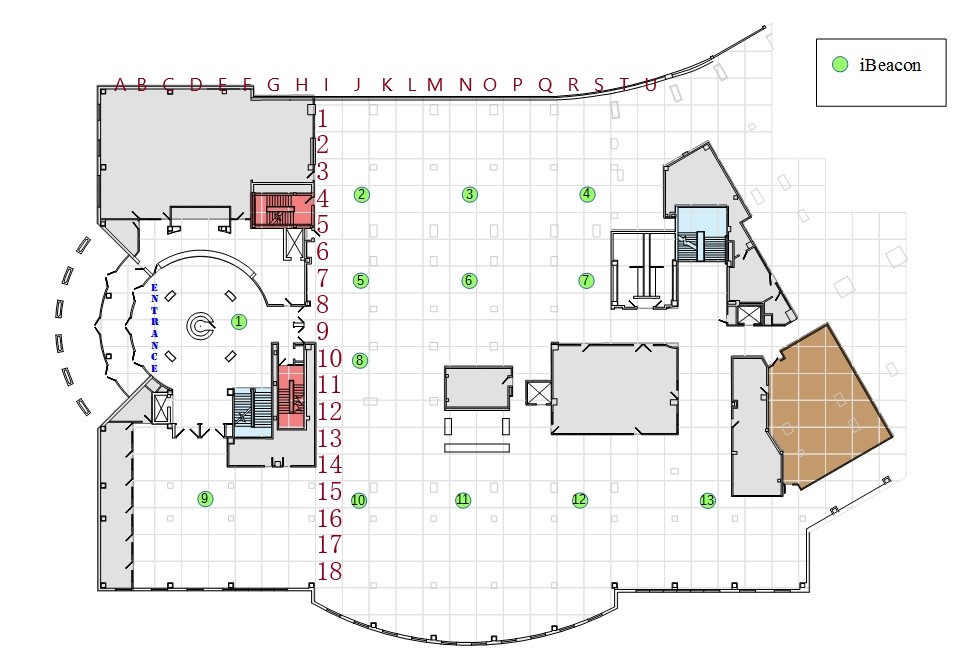
\includegraphics[width=1\textwidth]{./figures/ble_floor_layout.png}}
			\caption{Floor Layout for BLE dataset}
			\label{fig3.2}
			\end{figure}

			\subsubsection{Attribute Information}
				\begin{itemize}
				\item  \textbf{date:} Datetime in the format of ‘dd-mm-yyyy hh:mm:ss’
				\item  \textbf{b3001 - b3013:} RSSI numerical readings corresponding to the respective iBeacons.
				\item  \textbf{location:}The sites of acquiring RSSIs from iBeacons b3001 to b3013; representative numbers show the row and column of the site on the map (e.g., A03 stands for column A, row 3)
				\end{itemize}
	
			\subsection{Lab Dataset - Kaggle}
				One of the main challenges while deploying artificial intelligence for indoor localization is data acquisition. 
				We found few excellent datasets to perform our experiments. 
				We will use another dataset available on Kaggle, which corresponds to a lab in a university in India. 
				It contains only the information about the userID, the location of the user, and the RSSI values of the corresponding seven WAPs. 

			\subsubsection{Attribute Information}
				\begin{itemize}
				\item  \textbf{WAP001 – WAP 007:}  RSSI readings the corresponds to the respective WAPs; numeric.
				\item  \textbf{location:} The location of receiving RSSIs from WAPs. There are four unique locations in total
				\end{itemize}



	\chapter{Methodology}
		\section{Exploratory Data Analysis}
			Exploratory data analysis is a necessary part of the artificial intelligence scientific process.
			Engrossing visualizations assist scientists in comprehending their data and communicate their insights to their peers. ~\cite{Exploratory-data-analysis}.
			Tools can further progress these insights by specifying graphs that provide an appropriate balance between flexibility and efficacy.
			The matplotlib~\cite{4160265} project developed in python is highly flexible, offering fine-grained control over the exploration of various features of the dataset.
			Moreover, the seaborn~\cite{waskom2021seaborn} library offers an interface to matplotlib that permits prototyping of visualizations and rapid data exploration while retaining much of the flexibility and stability necessary to produce publication-quality graphics.

			We have utilized the expressiveness of these libraries to explore the richness of various features of our primary dataset.
			We created various plots and a storyboard to see how these features can be utilized in different applications. 
			The location of various users while collecting the data corresponds directly to the shape of the building, as depicted in figure~\ref{fig4.1}
	
	
			\begin{figure}[!htb]
			\centerline{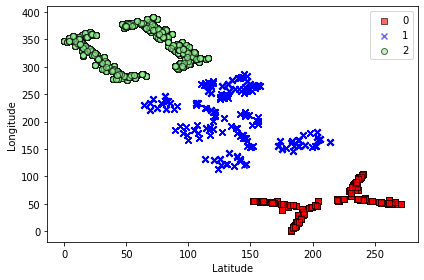
\includegraphics[width=0.8\textwidth]{./figures/building scatter plot.png}}
			\caption{Location of users while taking the observations}
			\label{fig4.1}
			\end{figure}
	
			Initially, we observed the number of users used in the collection of data over four months.
			We see in figure~\ref{fig4.2} that, in total, 18 users collected the data during the training phase, while identification of users was kept hidden during the validation phase. 
			The number of observations varied amongst the users with an average of 1107.6 observations, while the most readings taken by a user were 4516.
	
			\begin{figure}[h!]
			\centerline{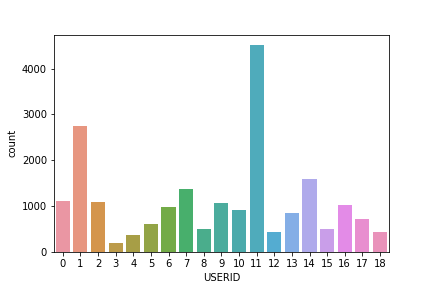
\includegraphics[width=0.7\textwidth]{./figures/user_id_count_plot.png}}
			\caption{Number of observations by each user}
			\label{fig4.2}
			\end{figure}
	
			As evident in figure~\ref{fig4.3}, twenty five different android phones were used to collect the data during the training phase to make a diversified dataset. 
			Two phones HTC Wildfire and LT22i~\cite{ujiindoor-data}, took the most readings with over 4500 observations.
			We also observed whether each user used a single phone or multiple phones and as it turned out that phone id 14 (LT22i) was used by three different users 1, 9, and 16.
	
	
			\begin{figure}[h!]
			\centerline{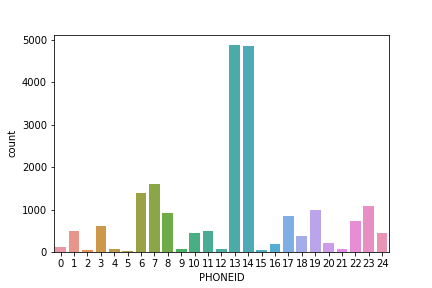
\includegraphics[width=0.7\textwidth]{./figures/phone_id_count_plot.png}}
			\caption{Number of observations by each phone}
			\label{fig4.3}
			\end{figure}
	
			There are three buildings in Universitat Jaume I (UJI) where these observations were taken. 
			Each of these buildings had multiple floors, and on analyzing the observations, we found that building 2 had the most number of observations during the training phase. 
			In the figure~\ref{fig4.4}, we can get insights about the distribution of observations among these floors and see that building 2 has five floors while the other two buildings have only four floors.
	
			\begin{figure}[h!]
			\centerline{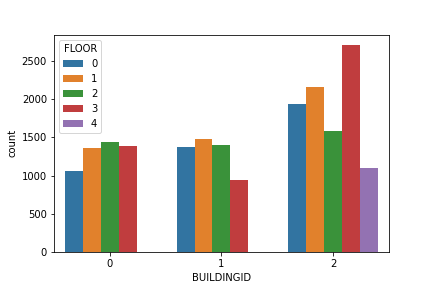
\includegraphics[width=0.7\textwidth]{./figures/floor_by_building_count_plot_training.png}}
			\caption{Number of observations taken on each floor of buildings}
			\label{fig4.4}
			\end{figure}
	
			Next, we looked into the distribution of the availability of WiFi access points (WAPs). 
			There were 520 WAPs in total in these buildings.  
			As depicted in the figure~\ref{fig4.5}, the access distribution of these WAPs is right-skewed, where the peak is around 15-18 WAPs. 
			This insight is significant to consider optimizing the access of WAPs for the users in indoor spaces.
	
			\begin{figure}[h!]
			\centerline{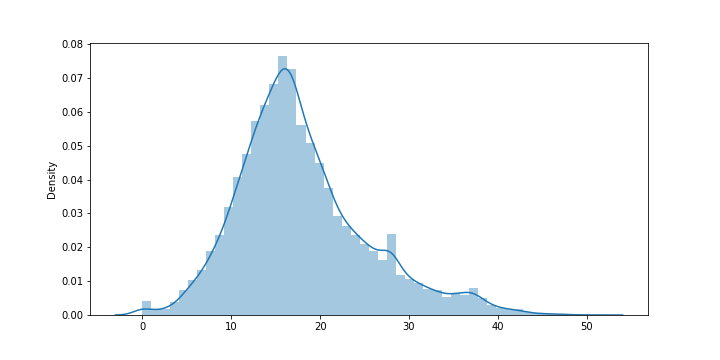
\includegraphics[width=0.7\textwidth]{./figures/wap_dist_plot.png}}
			\caption{Number of WAPs detected by each user reading}
			\label{fig4.5}
			\end{figure}
	
			Looking into these insights from a different perspective, we also tried to analyze the distribution of strength of the RSSI signals to different users, and it was found that similar to the access distribution of WAPs, this is also a right-skewed distribution. 
			As visible in the figure~\ref{fig4.6}, 71.12\% of non-null detection are in range [-95, -73] dB, which could also assist in the optimization of the distribution of WAPs.
	
			\begin{figure}[h!]
			\centerline{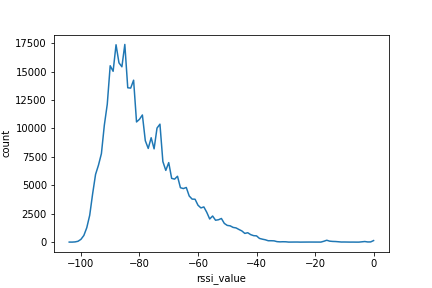
\includegraphics[width=0.7\textwidth]{./figures/rssi_distribution.png}}
			\caption{Strength of WAPs signals detected by each user reading}
			\label{fig4.6}
			\end{figure}
	
			One of the most exciting applications of indoor localization is its utility in indoor marketing. In shopping malls and other indoor complexes, it is vital to count the footfall of customers in different parts of the building. 
			The SPACEID in our data refers to the type of room in the building, for example, classroom, toilet, office, etc.
			We investigated the data from two perspectives to get insights. We investigated the number of unique visitors visiting a specific SPACEID and tried to follow the user's trajectory. 
			In the figure~\ref{fig4.7}, we can observe the mean and standard deviation of unique visits to each SPACEID, and this information could be utilized in the real estate sector, marketing and sales reference. 
			For instance, when a brand wants to buy a shop in a shopping complex, these insights can be used to witness the footfall of the customers and select the most appropriate place for an outlet.
	
			\begin{figure}[h!]
			\centerline{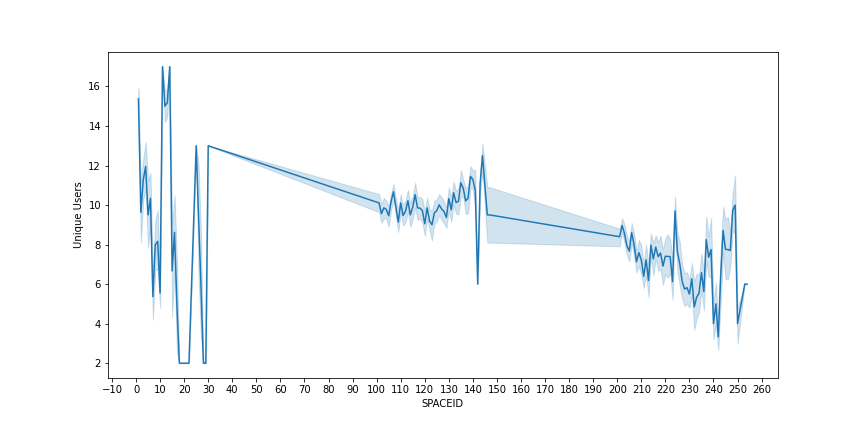
\includegraphics[width=1.2\textwidth]{./figures/user_by_spaceid_line_plot_training.png}}
			\caption{Number of Unique visits to a specific SPACEID}
			\label{fig4.7}
			\end{figure}
	
			Analyzing customers' behaviours using various methodologies of analysis with the secured data and providing them what they want, timely, would allow efficient operation of shopping malls~\cite{kim2015analysis}. 
			In this regard, keeping the animosity of the user, we can follow his trajectory. This tracking could assist in the optimization of the products and shops.
			In the figure~\ref{fig4.8}, we investigated the trajectory of User 11, who visited different floors of all three buildings. Here, we can see the trend of his visit and observe the amount of time he has spent on any floor. 
			This information could also be used together with market basket analysis which revolutionized the sales for different retailers like Merkur~\cite{svetina2005increase} uses market basket analysis throughout the promotion campaign process. 
			When a sales promotion is prepared, market basket analysis and user visit information can be used to define the right products and the right price for the campaign, increasing sales. 
	
			\begin{figure}[!htb]
			\centerline{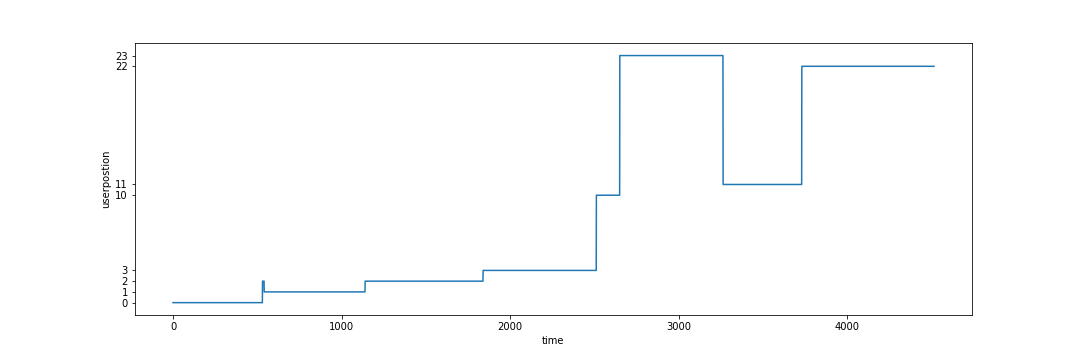
\includegraphics[width=1.2\textwidth]{./figures/user11_by_building_plot_training.png}}
			\caption{Trajectory of a Specific User}
			\label{fig4.8}
			\end{figure}
	
\newpage


		\section{Modelling as a Classification Problem}

		While exploring the dataset, we have observed that there could be multiple ways of localizing the personnel in the building. 
		We can use the coordinates values to locate the floor id, building id, and space id to predict location using this WiFi fingerprinting. 
		We would explore all these various approaches and study the behavior of different machine learning modeling techniques. 
		Initially, we will treat this problem as a classification problem and try to classify the building, floor, and room in which a user is present at that particular time. 
		We should respect that the validation dataset does not contain the SPACEID, so we would only look into the training dataset and formulate a predictive model. 
		We already have some state-of-the-art results that we tried to beat successfully. 
		
		Our goal is to develop a system to help people navigate a complex, unfamiliar interior space on a college campus. 
		We want to investigate the feasibility of using WiFi fingerprinting to determine a person’s indoor location.  
		If a model meets or exceeds minimum specifications, it could be incorporated into a smartphone app for indoor localization on a college campus.
		The indoor location must be as precise as predicting within 10-15 feet of the indoor room, also defined as SpaceID within source data. Relative position, or whether an individual is outside or inside of the room, is unnecessary.

		Ideal performance metrics to achieve:
		\begin{itemize}

		\item Accuracy scores on test data reaches 85\% or higher
		
		\item Precision (accuracy of minority class) on test data reaches 85\% or higher
		
		\item Recall (coverage of minority class) on test data is 85\% or higher

		\item  F1 Score for multi-class problem achieves 85\% or higher
		
		\end{itemize}	


			\subsection{Feature Engineering}
			There are three features of importance which are BUILDINGID, FLOOR, and SPACEID. 
			We approach the problem in 2 different ways: the overall location classification and the classification in individual buildings. 
			We created a combination of all these three features and treated them with a single label. We observed that there are 735 different classes, or room locations, to predict. 
			The WiFi Access Points will serve as the independent variables during algorithm training. In this problem, we have ignored the other features like LATITUDE, LONGITUDE, SPACEID, PHONEID, and USERID.  

			We also used an RMSE metric to assess the performance of our models.
			For this metric, we created a reference dataset assigning specific coordinates to each location (SPACEID).
			In this, we merged the relative position of the observation and treated each SPACEID as a single location.
			We created an xy-coordinate reference by rescaling the latitude and longitude using their difference from the respective minimum values.  

			\subsection{Data Preprocessing}

			Data Processing is one of the essential steps in our model formulation. We have observed a significant loophole in the dataset, which could be improved to increase the efficiency of our models. 
			In the dataset, there are 520 WAPs, but we observed that only 465 amongst them are those which a user at least once detects.
			Similarly, out of 19937 observations, 19861 observations detect at least one WAP. 
			So, we remove the unnecessary features and data points to have better-preprocessed data for our model.
			
			Moreover, as discussed in the dataset description chapter, the RSSI value of undetected WAP in the original dataset was denoted as 100; we changed it to -105 to better align with the data. 
			This conversion is done because all the RSSI values were negative, and it made more sense to have the undetected WAPs at the same end of the scale. 
			After replacing these values, we rescaled all the RSSI values to a positive scale to improve their interpretability, and models like Multinomial Naïve Bayes deal only with positive numbers.

			Another improvement that we made in the raw data is removing the noise using the z-score outlier detection methodology\~cite{eidleman1995z}. 
			The anomalies in the normally distributed data can be quantified using the statistical measurement of z-score.
			It calculates the number of standard deviations of each data point with respect to the mean of data.
			We took all the features independently and removed the outliers by taking three standard deviations criteria for detecting outliers. 

			\subsection{Feature Selection and Sampling}

			Redundant, irrelevant, and noisy features can be removed from the data with the help of feature selection techniques. It works as a dimensionality reduction technique and produces a subset of more relevant features from the raw data. 
			This process can improve the quality of the data leading to improved learning performance, lower computational cost, higher learning accuracy, and better model interpretability.
			Feature selection is based on the terms of feature relevance and redundancy concerning the goal of the machine learning process.
			
			For our use case, we created eight sub-datasets to access the performance of various machine learning models on them. 
			We created unprocessed and preprocessed datasets for each building as well as the whole dataset. 
			There was a high number of redundant features in these subsets. 
			For example, there are variables with only a single value of 0, aka zero variance variables. 
			The data description tells us a value of 0 indicates no WiFi signal detection; therefore, columns with a single observation or value (0=no signal detection) are most likely useless for modeling. 
			We observe a significant dimensionality reduction while creating building-wise datasets. 
			After this feature selection, for instance, we observed that building 0 dataset has only 5249-row observations with 200 WAP columns (Independent Variables) and 1 Location column (Dependent Variable).


			\subsection{Classification Model Selection}
				The procedure of selecting one ultimate machine research model from several candidates to achieve a training dataset is called model selection.
				 This procedure may be tried with several models, for example, logistic regression, SVM, KNN, etc.) also similar kind models organized with dissimilar model hyperparameters, for example, different kernels in an SVM.
				 We might want to augment a categorization or predictive regression model, and we can have a dataset for this purpose.
				 We have no idea the model which will be best suited to address this problem. So we try to discern between different models on this issue. 
				
				The top method to model selection calls for adequate data, which might be almost limitless depending upon the issue's complications.
				 In these hypothetical circumstances, we can break the data training, validation, and test sets, fit candidate models on the training set, assess and choose them on the validation set, and account for the functioning of the ultimate model on the test set.
				 This approach will be inappropriate on the most likely occurring modeling issues; we seldom have adequate data or can even determine what might be adequate.
				 Alternatively, there are two main ways to approach the hypothetical situation of choosing a model, they are :
				
				\begin{itemize}
				
				\item Probabilistic Measures: Choosing the model taking into consideration sample error and complications
				
				\item Resampling Methods: Choosing the model taking into consideration calculated out-of-sample inaccuracy
				
				
				\end{itemize}	
				
				
				\textbf{Probabilistic measures} include systematically gaining a candidate model by considering the complication of the model and conduct on the training dataset. 
				The training inaccuracy is overestimated. 
				Hence it cannot be used to select a model. 
				The performance may be handicapped depending on how much optimistic the training error is. 
				This methodology is commonly attained by utilizing algorithm-specific techniques, often linear, which will disrupt the result depending on the complication of the model.
				
				\textbf{Resampling methods} are used to calculate the conduct of a prototype (or, more accurately, the developing model procedure) on out-of-sample data. 
				This method is carried out by breaking the guidance dataset into sub train and test sets, fitting a model on the sub train set, and calculating it on the test set. 
				The specific technique can be carried out several times, and the average conduct for every test is revealed. 
				It will be a kind of Monte Carlo approximation of exemplary conduct on out of sample data; Even though every test in not solely independent, some data might reappear again and again in diverse training datasets or test datasets.
				
				Three standard resampling model selection methods include:
				
				\begin{enumerate}
				  \item Bootstrap~\cite{kohavi1995study}.
				  \item Cross-Validation (k-fold, LOOCV, etc.)~\cite{browne2000cross}.
				  \item Random train/test splits.
				\end{enumerate}
				
				
				A research method to assess model training prototypes on a finite data sample is referred to as \textbf{Cross-validation}. 
				This process will have one parameter referred to as k that refers to the different types of subsets in which one specified data sample is broken. 
				The specific process is referred to as k-fold cross-validation. 
				When one precise evaluation for k is considered, it can be used instead of full training set for the model; for instance, k=10 becomes 10-fold cross-validation which involves both training and holdout datasets. .

				For our use case, we perform the model selection by training eight different machine learning models using sklearn~\cite{sklearn-api} on all the unprocessed and preprocessed datasets. 
				Moreover, we have used cross-validation as a criterion for choosing the best two models based on accuracy as a selection metric. The machine learning models that we assessed are as follows: 
				\begin{enumerate}
				\item Decision Tree~\cite{quinlan1986induction,rokach2005decision}
				\item Random Forest~\cite{breiman2001random,liu2012new,livingston2005implementation}
				\item Support Vector Machines RBF~\cite{steinwart2008support,hearst1998support,campbell2011learning,liu2011feature}
				\item K Nearest Neighbors~\cite{goldberger2004neighbourhood, kramer2013k,zhang2016introduction}
				\item Multinomial NB~\cite{10.5555/1394399,kibriya2004multinomial}
				\item MLP Classifier~\cite{hinton1990connectionist, }
				\item LGBMClassifier~\cite{alzamzami2020light}
				\item LogisticRegression~\cite{dreiseitl2002logistic}
				\end{enumerate}


			\subsection{Classification Model Tuning}

				The points of options or layouts that will enable a machine learning model made for a particular task or dataset are called hyperparameters. 
				Machine learning models will have specifications that will be enhancing the model on an experimental dataset or the internal values adjusted by training.
				Parameters and hyperparameters are two different terms. Parameters will be acquired instinctively; hyperparameters are placed physically to assist in steering the research procedure. 
				
				Typically there will be a considerable consequence on a model of hyperparameter in the broader sense; however, it is unclear how to position a hyperparameter for a particular dataset. 
				A significant number of machine learning models will have a set of hyperparameters that will interrelate in nonlinear methods. 
				It is often essential to look for a set of hyperparameters that will lead to the optimum working of a model on a dataset. 
				This process is referred to as hyperparameter optimization, hyperparameter tuning, or hyperparameter search. 
				
				A definite exploration room is needed for the optimization process. 
				Search space is defined as volume to be searched in which every dimension denotes a hyperparameter, and every point represents one model configuration. 
				This procedure geometrically can be defined as an n dimension volume, in which each hyperparameter holds for a separate dimension. 
				The magnitude of the dimension is the rate that the hyperparameter will take. It can be whole-valued, categorical, or real-valued. 
				The exploration room will have a vector with an individual value for every hyperparameter. 
				This process aims to find the vector that will bring about the optimum conduct of the model after learning, like the highest accuracy or lowest error.
				
				The various optimization algorithm can be taken; the most straightforward out of these are two :
				
				\begin{itemize}
				
				\item \textbf{Random Search}: Allocate an exploration room as an enclosed realm of hyperparameter evaluations and arbitrarily sample points in that area.
				\item \textbf{Grid Search:} Define a search space as a grid of hyperparameter values and evaluate every position in the grid.
				
				\end{itemize}	
				
				
				\textbf{Grid search} is optimum for evaluating spot combinations that are investigated to conduct better. 
				\textbf{Random search}  is excellent for finding new hyperparameter combinations which cannot be figured out instinctively. 
				However, the time needed for it to execute is longer than for grid search.  
				For our specific use case, we have used both hyperparameter optimization algorithms. 
				For Random Forest, we used random search optimization, and for support vector machines, we used the grid search cross-validation optimization. 
				We have deployed these optimization algorithms on the processed data for the entire data set and each building separately.

			\subsection{Metrics for Evaluation of Results}

				Model selection is choosing one of the models as the final model that addresses the problem. 
				Model selection is different from model assessment.
				For example, we evaluate or assess candidate models to choose the best one, which is model selection. 
				Once a model is chosen, it can be evaluated to communicate how well it is expected to perform in general; this is model assessment.
				
				The metrics that we choose to evaluate our machine learning algorithms are essential. 
				Choice of metrics influences how the performance of machine learning algorithms is measured and compared. 
				They influence how we weigh the importance of different characteristics in the results and our ultimate choice of which algorithm to choose. 
				For our use case, we decided to evaluate the performance of our hyperparameter optimized models against six different evaluation metrics. 

				\begin{itemize}
				\item Accuracy: $ \text{accuracy} = \frac{\text{true positives} + \text{true negatives}}{\text{true positives} + \text{false positives} + \text{true negatives} + \text{false negatives}}$
				\item Precision: $ \text{precision} = \frac{\text{true positives}}{\text{true positives} + \text{false positives}}$
				\item Recall: $ \text{recall} = \frac{\text{true positives}}{\text{true positives} + \text{false negatives}}$
				\item F1 Score: $ \text{F1} = \frac{2 \times \text{precision} \times \text{recall}}{\text{precision} + \text{recall}}$
				\item MSE: $mean\_square\_error = \frac{\sum (\text{true\_value} - \text{predicted\_value})^2}{\text{N}}$
				\item MSE (Incorrect Predictions Only)
				\end{itemize}
				
				MSE is the distance between the real SPACEID and predicted SPACEID. We have used the latitude and longitude associated with each SPACEID to create this custom evaluation metric. 

			\subsection{Evaluation of PCA on full data}
				Reducing the number of input variables for a predictive model is referred to as dimensionality reduction. 
				Fewer input variables can result in a simpler predictive model with better performance when making predictions on new data~\cite{howley2005effect}.
				Perhaps the most popular technique for dimensionality reduction in machine learning is Principal Component Analysis, or PCA for short. 
				This technique comes from the field of linear algebra and can be used as a data preparation technique to create a dataset projection before fitting a model. 
				It can be thought of as a projection method where data with m-columns (features) is projected into a subspace with m or fewer columns whilst retaining the essence of the original data.
				
				The PCA method can be described and implemented using the tools of linear algebra, specifically a matrix decomposition like an Eigendecomposition or SVD. 
				We have applied PCA on our full dataset and evaluated the performance of the Random Forest model on 20\%, 40\%, 60\%, 80\%, and 100\% of the data to observe how the curse of dimensionality affects our model.



\newpage


		\section{Modelling as a Regression Problem}
			\subsection{Feature Engineering}

			Feature engineering is the process of transforming raw data into features that better represent the underlying problem to the predictive models, resulting in improved model accuracy on unseen data. 
			As in the previous case of modelling as a classification problem, we would remove the redundant observations where the user detected no WAPs. 
			We would also remove the features which a user did not detect during the training phase. 
			We must note that here, the validation data set also contains information about the latitude and longitude of the user, so we will use complete training data for training and then test it on the validation data.
			
			The latitude and longitude in our problem are given as UTM coordinates. 
			UTM stands for “Universal Transverse Mercator”. 
			It is a geographic coordinate system used to identify locations on earth in meters, as measured in the Northern Hemisphere going North and East from the intersection of the equator and a central meridian assigned to each of 60 longitudinal zones around the earth. 
			We would rescale these latitude and longitude values to xy-coordinates, where we take the difference of each value with the minimum of its respective latitude and longitude in our data set. 

				\subsubsection{RSSI Signal Strength to Distance}

				To treat this as a regression problem, we need to transform our features from the RSSI dB scale to the Linear scale. 
				In our raw dataset, all the WAPs values are in the RSSI scale. 
				RSSI stands for Received Signal Strength Indicator, which is the strength of the access point`s signal seen on the receiving device, e.g. a smartphone. 
				The signal strength depends on distance and Broadcasting Power value. At maximum Broadcasting Power (+4 dBm), the RSSI ranges from -26 (a few inches) to -100 (40-50 m distance).
				
				RSSI is used to approximate the distance between the device and the access point using measured power defined by the WAPs standard. 
				Measured power is a factory-calibrated, read-only constant that indicates the expected RSSI at a distance of 1 meter to the access point. 
				Combined with RSSI, it allows estimating the distance between the device and the access point. 
				While defining the conversion formula, we also need to consider a constant N that depends on the environmental factor (range 2-4).

				\[Distance = 10^{\frac{(Measured Power - RSSI)}{10N}}\]
				
				Measured power is also known as the 1 Meter RSSI. 
				For our use case, we took the value of measure power as -60 and considered N as 3. 
				This power means that when our value of RSSI is -60, the distance between the user and access point is 1 meter and it increases as the signal strength (RSSI) decreases according to the formula given above.

			\subsection{Feature Selection and PCA}

				As explained earlier, PCA is a simple dimensionality reduction technique that applies linear transformations to the original space. 
				Among all the orthogonal linear projections, PCA minimizes the reconstruction error~\cite{jablonski2015principal}, the distance between the instance and its reconstruction from the lower-dimensional space. 
				That is the sum of the distances between points in the original space and the corresponding points in lower-dimensional space.
				A critical point to mention is that PCA is an unsupervised form of dimensionality reduction.
				This form means the response variables are not taken into consideration at any point of the transformation. 
				
				Principal component analysis~\cite{wold1987principal} of a data matrix extracts the dominant patterns in the matrix in terms of a complementary set of score and loading plots. 
				For plotting purposes, two or three principal components are usually sufficient, but for modelling purposes, the number of significant components should be adequately determined, e.g., by cross-validation.
				As shown in figure~\ref{fig4.9}(a), the first 150 eigenvectors explain Roughly 95\% of the variance. 
				Before we perform the dimensionality reduction on our data, we also analyzed the reconstruction error as a function of the dimensions.
				
				As the number of principal components used for the reconstruction increases, the reconstruction error expectedly decreases. 
				This figure ~\ref{fig4.9}(b) is a mirror image of the previously explained variance ratio figure.
				As 95\% of the variance is explained by the top 150 components, we reduced our training and test data to 150 dimensions.
				
				\begin{figure}[h!]
				  \centering
				  \begin{subfigure}[b]{0.48\linewidth}
				    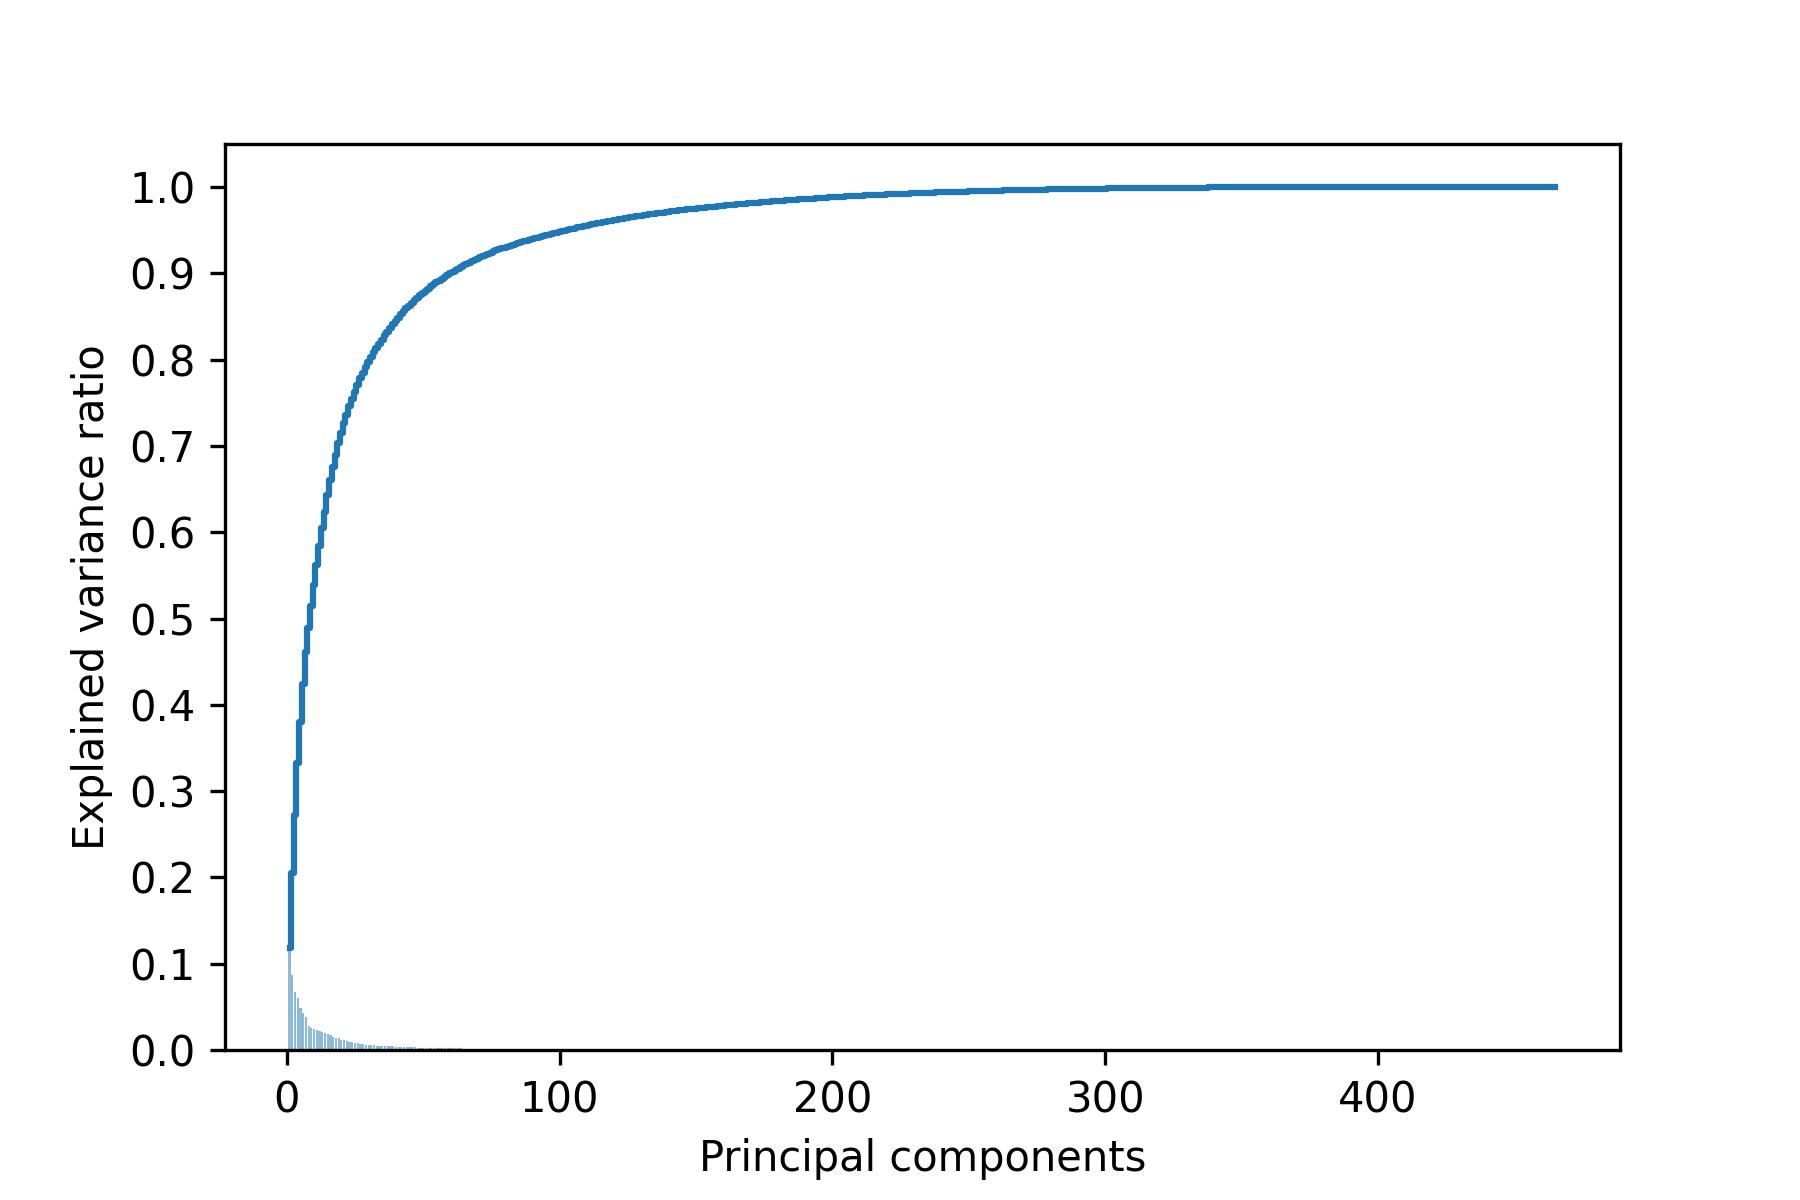
\includegraphics[width=\linewidth]{./figures/pca.explained_variance_ratio_.png}
				     \caption{Explained Variance Ratio}
				  \end{subfigure}
				  \begin{subfigure}[b]{0.48\linewidth}
				    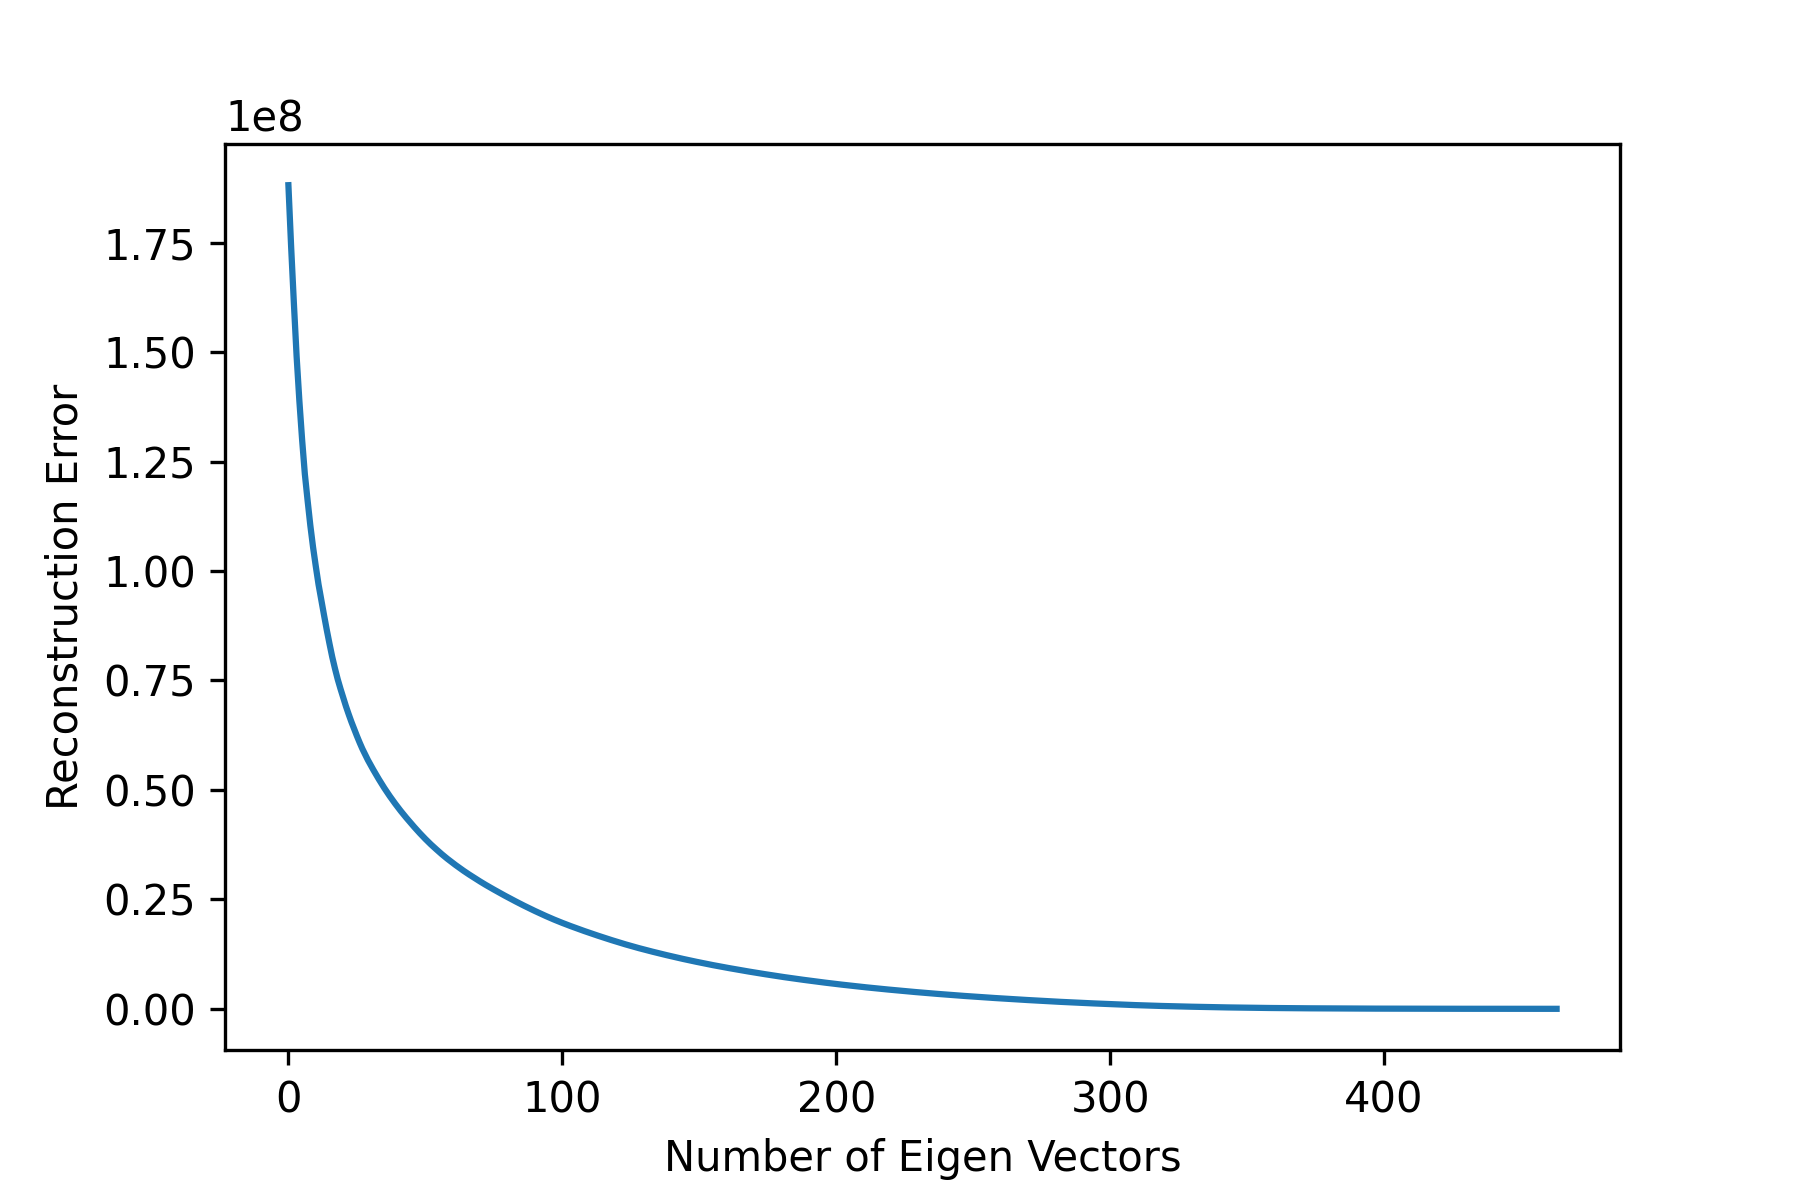
\includegraphics[width=\linewidth]{./figures/pca.Reconstruction Error.png}
				    \caption{Reconstruction Error}
				  \end{subfigure}
				  \caption{PCA of training data set}
				  \label{fig4.9}
				\end{figure}
				
				In figure~\ref{fig4.10}, we illustrated how the BuildingID are distributed across the top two PCA dimensions. It is significantly visible that these top two PCA components depict a stratification amongst the three buildings. 
				Remember PCA is an unsupervised learning technique for dimensionality reduction. 
				So, it is quite possible the two top PCA components might not have explained our response variable well.
				
				
				
				
				\begin{figure}[!htb]
				\centerline{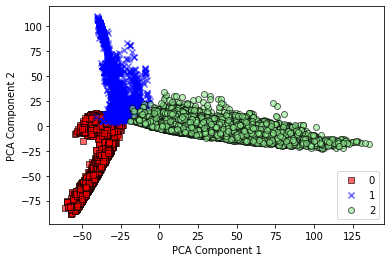
\includegraphics[width=0.8\textwidth]{./figures/pca components distribution.png}}
				\caption{Distribution of PCA components}
				\label{fig4.10}
				\end{figure}

			\subsection{Regression Model Selection}
				Multivariate regression~\cite{alexopoulos2010introduction,izenman2013multivariate} is used to measure how more than one independent variable (predictors) and more than one dependent variable (responses) are linearly related.
				The method is broadly used to predict the behavior of the response variables associated with changes in the predictor variables once a desired degree of relation has been established. 
				As our model should predict both latitude and longitude of the user, we will train a multivariate regression model.
				As discussed in the modelling of classifiers, we will use the nested cross-validation method to assess the performance of our models for model selection. 
				We performed nested cross-validation on the different model families. 
				In nested cross-validation, the inner fold performs the parameter tuning, and the outer fold is used for validation. 
				We used linear regression models, polynomial regression models, and some other non-linear regression models for selection.
				 
				The fundamental concepts of building the regression framework include:
				\begin{itemize}
				\item \textbf{MultiOutputRegressor:} We have the model response as a vector of 2-dimensions (Latitude and Longitude). 
				Not every regression method in scikit-learn can handle this sort of problem. 
				Most linear models provide this capability, but a new class MultiOutputRegressor is available for parallelization of regressors for multivariate output for those that do not.
				\item \textbf{Linear Regression Models:} First, we focussed on Linear regression and its variants, including Lasso~\cite{zhang2008sparsity}, Ridge Kernels~\cite{mcdonald2009ridge}.
				\item \textbf{Polynomial Features:} Considered Polynomial Features including quadratic~\cite{ostertagova2012modelling} and cubic for addressing non-linearities.
				\item \textbf{Other Regression Models:} K-Nearest Neighbour~\cite{goldberger2004neighbourhood, kramer2013k,zhang2016introduction}, ExtraTreesRegressor~\cite{geurts2006extremely}, and RandomForestRegressor~\cite{segal2004machine}.
				\end{itemize}
				
				We will train and perform machine learning model selection for the whole dataset as well as for each floor-building dataset individually as well.
				
							\subsection{Regression Model Tuning}
				
				Tuning is the process of maximizing a model's performance without overfitting or creating too high of a variance. 
				As explained earlier, in machine learning, this is accomplished by selecting appropriate "hyperparameters." 
				We considered the best-performing model from the model selection process and then used the grid search cross-validation process to find the best hyperparameters for our model.
				While tuning, we also took insights on how an increase in the training data corresponds to the training and validation loss. 
				We gradually increased the size of the training and evaluated its performance, as shown in the figure~\ref{fig4.11}. 


				\begin{figure}[h!]
					\centering
					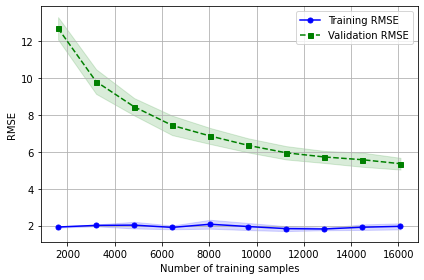
\includegraphics[width=0.8\linewidth]{./figures/learning_curve.png}
					\caption{Learning curve for optimized regressor}
					 \label{fig4.11}
				\end{figure}

\newpage


		\section{Modelling as a Multi Cascaded Classification and Regression Problem}
			\subsection{Three Stage Cascaded Machine Learning Model}

			In these experiments, we will make use of the models explained in the prior sections. 
			We developed a three-stage multi-cascaded machine learning model to predict user location based on the dataset's building, floor, latitude, and longitude information. 

				\subsubsection{Classifier For Building Prediction}

					In the first stage of the cascaded model, we integrated a classifier that predicts the BuildingID of the user. 
					We used the best model according to the assessment done in the modelling of the classification model section.

				\subsubsection{Classifier For Floor Prediction}
					In the second stage of the cascaded model, we will utilize the information in the dataset, and the BuildingID predicted in stage one to predict the user's floor. 
					Initially, we developed a global floor classifier, but its performance was evaluated to be less accurate. 
					However, adding the information of the BuildingID, the performance of the model significantly increases.

				\subsubsection{Regressor For final Prediction}
					After stacking two classifiers, we integrated a multivariate regressor into the cascaded model to finalize it. 
					Again, we tested both the global regression models and the per floor per building regression problems, and we found that the performance of the global regression model is significantly better, so we proceeded with that. 

			\subsection{Metric for Evaluation of Results}
				The mean positioning error is expressed as the mean Euclidean distance between the actual and estimated locations. 
				However, in multi-building, multi-floor environments, as in our problem, just the positioning error due to Euclidean distance is not enough. 
				Wrong floor and wrong building classification are not desirable as the actual movement from the predicted location to the actual location might involve significant displacement.
				
				Therefore, we include penalty terms to the mean error equation to penalize floor and building classification failures. 
				This penalty term was introduced in the 2015 EvAAL-ETRI competition~\cite{torres2017realistic}. 
				The cost function can be expressed as follows:
				
				\begin{equation}
				  \begin{array}{l}
				 positioning\_error(actual,predicted)=euclidean\_distance(actual,predicted) \\
				+ penalty\textsubscript{floor}∗fail\textsubscript{floor}+penalty\textsubscript{building}∗fail\textsubscript{building}
				  \end{array}
				\end{equation}

				where  fail\textsubscript{floor}  and  fail\textsubscript{building} indicate if the floor and building are incorrectly identified,   penalty\textsubscript{floor}  and  penalty\textsubscript{building}  are the penalty values applied for wrongful classification of floor and building, respectively. 
				
				The penalty values were set to 4 and 50 respectively in the third track of the competition~\cite{potorti2015evaluating}. 
				Expectedly, the penalty for building classification failure is higher than that of floor classification failure. 



\newpage


		\section{Trilateration Methodology for localization of Access Points}

			The process of determining the relative or absolute location of points using geometrical measurement of distances is known as trilateration. 
			In trilateration, we analyze the geometry of triangles, circles, hyperboloids, or spheres to estimate our target's location. 
			Mathematically, this technique can be interpreted in terms of calculating the position of a point in space using the distances from the location of known geometrical entities.

			\subsection{Geometrical Interpretation}
				We can state the formulation in terms of a geometrical problem. 
				Let us consider a location of a point P in space, which would be a WiFi access point. 
				We can use the coordinates of a known location L of a user when he takes the RSSI reading for that specific WAP. 
				These locations, L and P, can be states in terms of latitude and longitude coordinates. 
				As explained in techniques for indoor localization, one source can only be used for proximate-based localization. 

				We can only estimate the proximity of access point P relative to the user's location L but not the exact distance in between them. 
				As shown in figure~\ref{fig4.12}, the user's device L creates a virtual circle around it regarding signal reception. 
				In 3D terms, it is a sphere, but we consider it a circle for our derivation. All the points on the circumference are potential candidates for the position of the WAP.

				\begin{figure}[htb!]
					\centering
					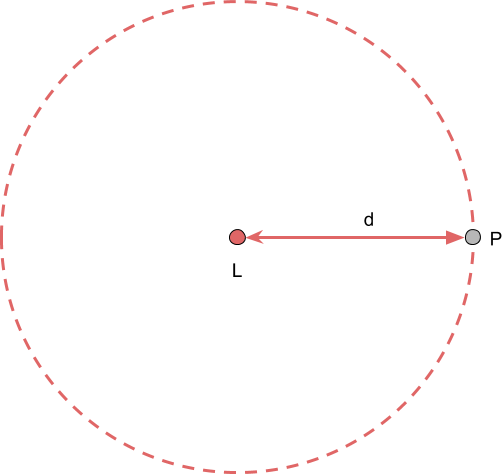
\includegraphics[width=0.35\linewidth]{./figures/Trilateration1.png}
					\caption{Trilateration using one points}
					 \label{fig4.12}
				\end{figure}
				
				We can improve the situation by inducing two users, $L_1$ and $L_2$, as shown in figure~\ref{fig4.13}. 
				Now, our access point P should be at the circumference of the green and red circles that originate from these two different users. 
				We can solve this in terms of the point of intersections of both these circles, which leads us to only two options, as shown in grey.

				\begin{figure}[htb!]
					\centering
					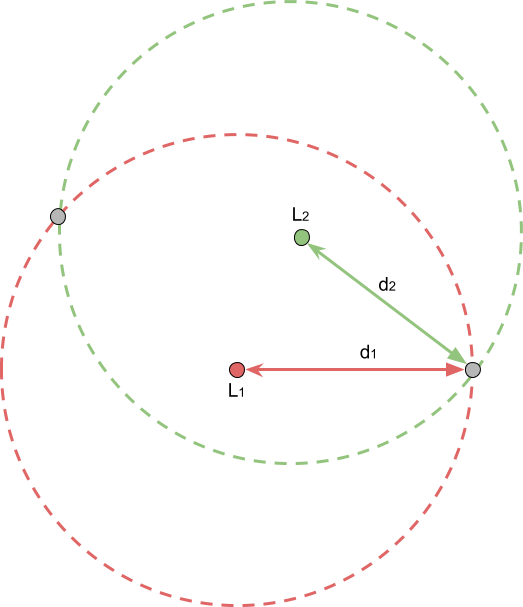
\includegraphics[width=0.35\linewidth]{./figures/Trilateration2.png}
					\caption{Trilateration using two points}
					 \label{fig4.13}
				\end{figure}
				
				To further improve the interpretation and move from proximity-based localization to distance-based localization, we introduce a third user, $L_3$, in our frame of reference. 
				As shown in figure~\ref{fig4.14}, we have three circles whose interference should contain the access point's location. 
				As interference of three circles is a single point in space, we can solve these circles to estimate the location P of WAP.
				
				\begin{figure}[htb!]
					\centering
					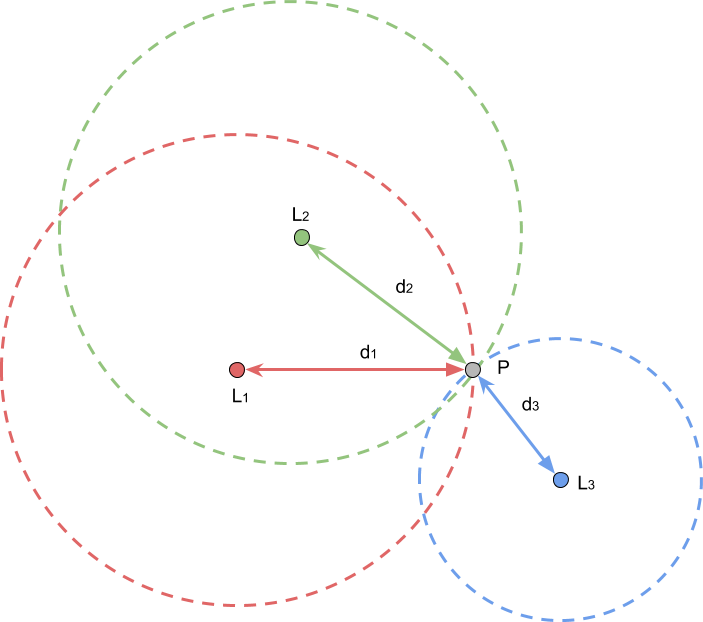
\includegraphics[width=0.35\linewidth]{./figures/Trilateration3.png}
					\caption{Trilateration using three point}
					 \label{fig4.14}
				\end{figure}

			\subsection{Mathematical Interpretation}

				We can solve these three circles in terms of mathematical equations. 
				The equation of circle provides us the position coordinates $\left(c_x, c_y\right)$  of the point $\left(x,y\right)$  present on the circumference of circle with diameter $d_1$.
				
				
				\[{\left(x - c_x\right)}^2 + {\left(y- c_y\right)}^2={d_1}^2\]
				
				
				This reasoning can be extended to the circles of signal reception created by all three users considered before. 
				Latitude and longitude coordinates, $\left(\phi_1, \lambda_1 \right)$, $\left(\phi_2, \lambda_2 \right)$ and $\left(\phi_3, \lambda_3 \right)$,  are used to express location of the three users respectively. 
				This leads us to the following resultant locations. 
				
				\[{\left(\phi - \phi_1\right)}^2 + {\left(\lambda- \lambda_1\right)}^2={d_1}^2\]
				\[{\left(\phi - \phi_2\right)}^2 + {\left(\lambda- \lambda_2\right)}^2={d_2}^2\]
				\[{\left(\phi - \phi_3\right)}^2 + {\left(\lambda- \lambda_3\right)}^2={d_3}^2\]
				
				This problem is now translated into the mathematical equation that can be simultaneously solved to provide the resultant interference point P=$\left(\phi, \lambda\right)$ for the three circles. 
			
			\subsection{Optimzation Algorithm}

				Ideally, the trilateration problem should be seen and solved in geometrical equations, but in reality, this does not always lead to practical solutions. 
				These three circles are not very precise in the real world, which could lead to a null solution if three circles do not intersect at a single point as mathematical modelling involves significantly high accuracy on our measurements. 
				Moreover, if the number of points in space is increased to a very high number, solving them simultaneously becomes less efficient, which would hinder our approach's scale. 
				In real life, there could be tens of users connecting a single WAP, and they all would contribute to estimating the WAP's location. 
				
				We can translate this mathematical problem to an optimization one. 
				We can ignore intersections and circles; focus on the point X=$\left(\phi_x, \lambda_x\right)$ that would lead us to the optimized approximation of the location of the respective access point. 
				
				Let us assume that we have a point X that can replace point P in space. 
				We can estimate its euclidean distance loss from point P by optimizing its distance $d_i$ from all the users $L_i$ under consideration. 
				X is at the same position as P if all the distances $d_i$ precisely match with the distances of access points from users available in the problem statement. 
				The further point P moves from X, the more is the deviation between actual and predicted distances. 
				
				We need to define a particular error function that should be minimized to treat trilateration as an optimization problem. 
				This error should be the difference between predicted and actual distances for all three users, which can be calculated using these three equations.
				
				 \[e_1 = d_1 - dist\left(X, L_1\right)\]
				 \[e_2= d_2 - dist\left(X, L_2\right)\]
				 \[e_3 = d_3 - dist\left(X, L_3\right)\]
				
				We can solve these errors in terms of mean squared error (MSE). MSE is calculated by taking an average of the squares of all the distance differences. 
				As squares are always positive, this approach reduces the error induced by the negative and positive distance differences.  
				We can sum up our work by defining the following formula optimized to estimate our target location.
				
				\[\frac{\sum { \left[d_i  -dist\left(X,L_i,\right)\right] }^2 }{N}\]


			\subsection{Implementation}

				We made use of the available information and this methodology to specify the location of the WAP. We take the following steps to apply the trilateration process:
				\begin{enumerate}
				\item We converted the signal strength from the RSSI dB scale to the linear distance scale while formulating a regression model. 
				The figure~\ref{fig4.15} shows the relationship between the signal strength and distance between a user and the access point.
				\item While treating it as an optimization problem, we need an initial guess for which we took the mean of the location of all the users that detected a specific WAP as this initial guess.
				\item We treated WAPs individually, and for each WAP, we considered only the users that detected that specific WAP. Then, we optimized the position of the WAP by taking a mean squared error loss concerning the distance from the user.
				\item Finally, we converted the location coordinates from the UTM scale to GPS for better visualization.
				\end{enumerate}
				
				
				\begin{figure}[h!]
					\centering
					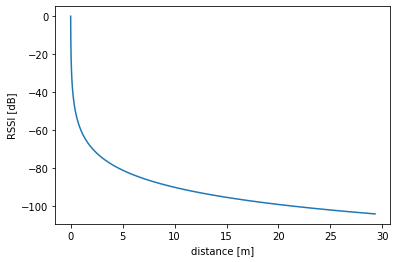
\includegraphics[width=0.7\linewidth]{./figures/Received signal strength vs distance.png}
					\caption{Relation between RSSI signal strength and distance}
					 \label{fig4.15}
				\end{figure}


	\chapter{Results}
		\section{Modelling as a Classification Problem}

			The first step of modelling a classifier was model selection. 
			As explained in the methodology, we deployed eight different classification models on datasets and evaluated their performance using five-fold cross-validation. 
			Here, our models were trained on a combination of building, floor, and space information as a label. 
			In figure~\ref{fig5.1}, we can see the comparison between these different machine learning models for both the unprocessed and preprocessed data. 
			We can see that the Random Forest model performs best for both the unprocessed and preprocess complete datasets. 
			The second best in Support Vector Machine model with RBF kernel. We have selected these two models and proceed with the model tuning process. 
			Here, we have used accuracy as a metric of assessment for the performance of models.
			
			\begin{figure}[!htb]
			  \centering
			  \begin{subfigure}[b]{0.48\linewidth}
			    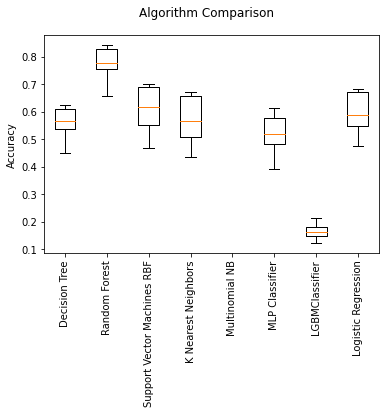
\includegraphics[width=\linewidth]{./figures/results_model_comparison_unprocessed_full_data.png}
			     \caption{Unprocessed full data}
			  \end{subfigure}
			  \begin{subfigure}[b]{0.48\linewidth}
			    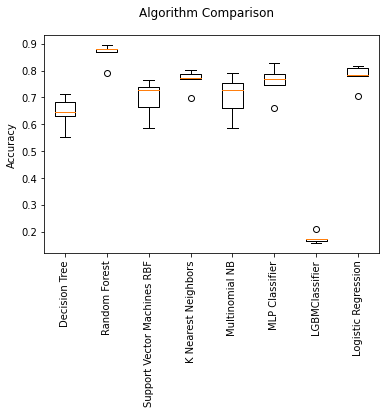
\includegraphics[width=\linewidth]{./figures/results_model_comparison_preprocessed_full_data_updated.png}
			    \caption{Preprocessed full data}
			  \end{subfigure}
			  \caption{Model selection for full data}
			  \label{fig5.1}
			\end{figure} 
			
			After the model selection for the whole dataset, we applied the same process of all three buildings individually and assessed the performance of eight non-linear machine learning classifiers. 
			In figure~\ref{fig5.2}, we can see the results for Building 0. 
			Here, we can see that the performance of all the models is generally worse for Building 0 data compared to the entire dataset for both the processed and unprocessed cases. 
			This observation could be related to the fact that we have the least number of user observations in Building 0 amongst all three buildings. 
			However, here again, Random Forest performs the best among all the classifiers. 
			
			\begin{figure}[!htb]
			  \centering
			  \begin{subfigure}[b]{0.48\linewidth}
			    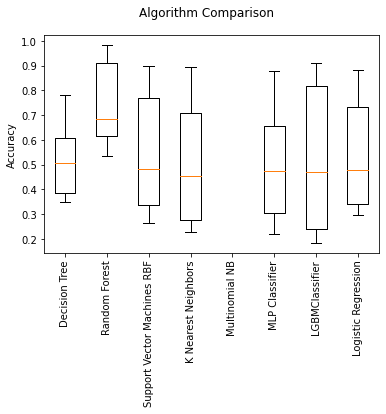
\includegraphics[width=\linewidth]{./figures/results_model_comparison_unprocessed_building0_data.png}
			     \caption{Unprocessed building 0 data}
			  \end{subfigure}
			  \begin{subfigure}[b]{0.48\linewidth}
			    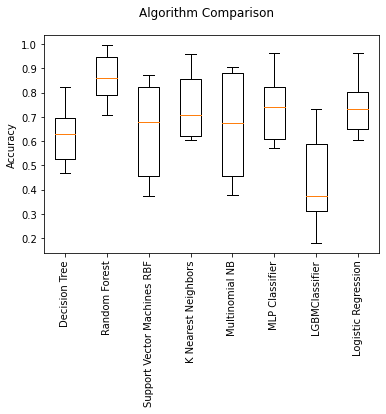
\includegraphics[width=\linewidth]{./figures/results_model_comparison_preprocessed_building0_data.png}
			    \caption{Preprocessed building 0 data}
			  \end{subfigure}
			  \caption{Model selection for building 0 data}
			  \label{fig5.2}
			\end{figure}
			
			In figure~\ref{fig5.3}, we can visualize the model selection process for Building 1. 
			We see an improvement in the model's overall performance compared to Building 0 and the entire dataset. 
			This insight corresponds to the fact that there are more data points for Building 1 than Building 0. 
			As visualized in figure~\ref{fig5.17}, the architecture of Building 1 is as such that there is greater segregation among the sectors of the building, and the area of Building 1 is significantly higher as well, which tends to lead to a better distribution of the data points. 
			
			
			\begin{figure}[!htb]
			  \centering
			  \begin{subfigure}[b]{0.48\linewidth}
			    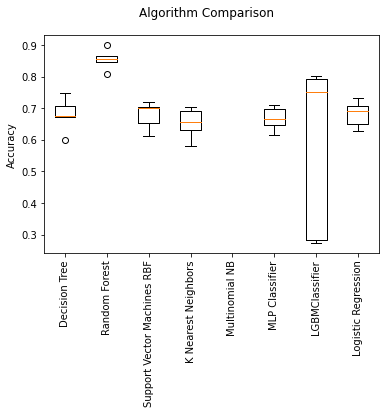
\includegraphics[width=\linewidth]{./figures/results_model_comparison_unprocessed_building1_data.png}
			     \caption{Unprocessed building 1 data}
			  \end{subfigure}
			  \begin{subfigure}[b]{0.48\linewidth}
			    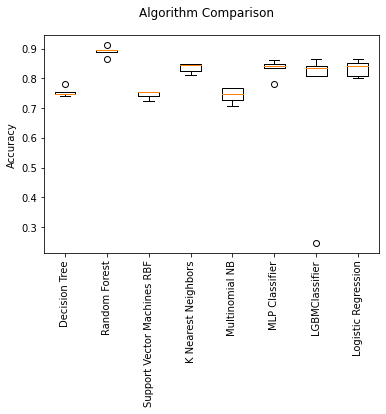
\includegraphics[width=\linewidth]{./figures/results_model_comparison_preprocessed_building1_data.png}
			    \caption{Preprocessed building 1 data}
			  \end{subfigure}
			  \caption{Model selection for building 1 data}
			  \label{fig5.3}
			\end{figure} 
			
			Finally, for the UJI Indoor dataset, figure~\ref{fig5.4} illustrates the performance of various machine learning algorithms for Building 2 datasets. 
			It can be seen that the performance here is also less as compared to the entire dataset for both unprocessed and preprocessed datasets. 
			This reduction in performance is highly due to a single floor of Building 2. 
			As illustrated in figure 4.4, building 2 has five floors while the other two buildings have four floors each. 
			The 5th floor of the building had the least number of observations amongst all the floors, and on analysis of individual floors, it was found that the classifier's performance on this specific floor is worse than the rest. 
			Hence, this floor reduces the overall performance of the models on Building 2. 
			It must also be observed that the Multinomial NB does not work for unprocessed data as it requires positive values for independent variables, whereas our unprocessed data contains negative RSSI values. 
			
			\begin{figure}[!htb]
			  \centering
			  \begin{subfigure}[b]{0.48\linewidth}
			    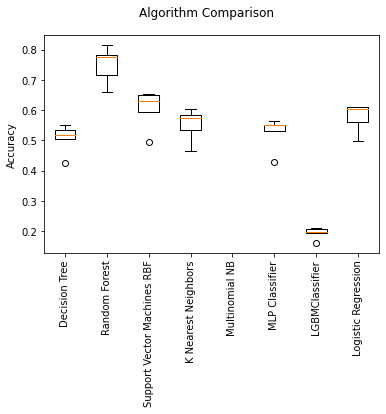
\includegraphics[width=\linewidth]{./figures/results_model_comparison_unprocessed_building2_data.png}
			     \caption{Unprocessed building 2 data}
			  \end{subfigure}
			  \begin{subfigure}[b]{0.48\linewidth}
			    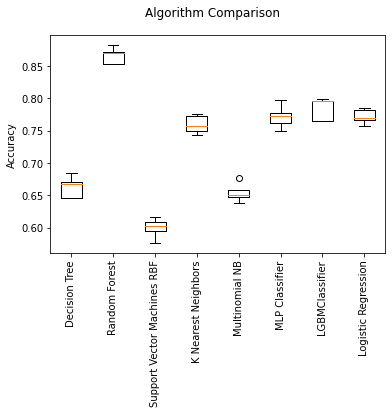
\includegraphics[width=\linewidth]{./figures/results_model_comparison_preprocessed_building2_data.png}
			    \caption{Preprocessed building 2 data}
			  \end{subfigure}
			  \caption{Model selection for building 2 data}
			  \label{fig5.4}
			\end{figure} 
			
			In order to generalize our study of machine learning techniques, we also performed a model selection of two other independent datasets. 
			In figure~\ref{fig5.5}, we can see the performance of machine learning models on the BLE data set, which was collected in Waldo Library, Western Michigan University. 
			The performance of our machine learning models is abysmal on this dataset. 
			It ranges around 0.35 for the best performing Random Forest model.  
			This accuracy score can be explained by taking insights from the layout of the floor library, as illustrated in figure~\ref{fig3.2}. 
			
			The data is collected iBeacons whose range is significantly less than the WiFi access points, so they do not cover a large area, and the particular importance of an iBeacon reduces in context to the whole floor.
			Moreover, the locations are taken from the grid presented in the layout.
			Each location is a cartesian product of row and column, and as can be seen, there is no clear separation between the locations, and they are mostly intermingled, so the prediction for the artificial intelligence system gets worse in this case.
			
			\begin{figure}[!htb]
			  \centering
			  \begin{subfigure}[b]{0.48\linewidth}
			    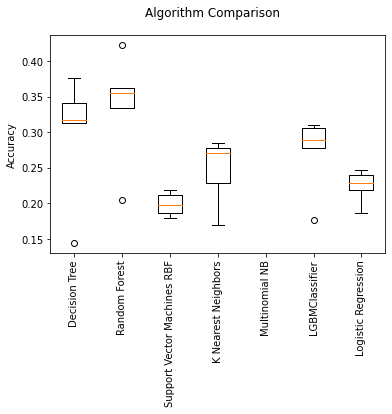
\includegraphics[width=\linewidth]{./figures/results_model_comparison_unprocessed_full_data_ble.png}
			     \caption{Unprocessed full data}
			  \end{subfigure}
			  \begin{subfigure}[b]{0.48\linewidth}
			    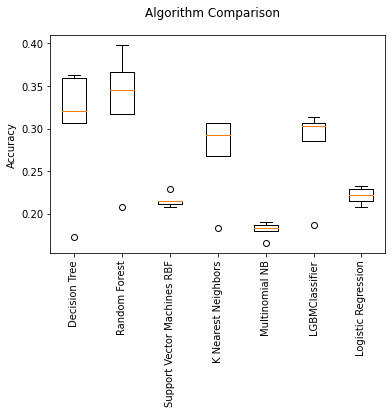
\includegraphics[width=\linewidth]{./figures/results_model_comparison_preprocessed_full_data_ble.png}
			    \caption{Preprocessed full data}
			  \end{subfigure}
			  \caption{Model selection for BLE data}
			  \label{fig5.5}
			\end{figure} 
			
			Finally, to establish our point that better segregation of locations leads to better performance of the AI system, we performed the model assessment of another lab data.
			Here, we only have 4 locations and 1500 readings for seven different access points. 
			Here in figure~\ref{fig5.6}, we see that the performance is very high for both the unprocessed and preprocess datasets.
			This insight again lays down the importance of the excellent quality data acquisition process for indoor localization.
			
			\begin{figure}[!htb]
			  \centering
			  \begin{subfigure}[b]{0.48\linewidth}
			    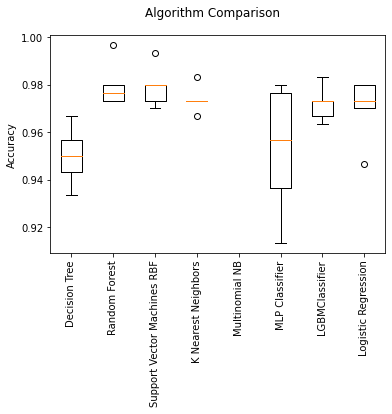
\includegraphics[width=\linewidth]{./figures/results_model_comparison_unprocessed_full_data_lab.png}
			     \caption{Unprocessed full data}
			  \end{subfigure}
			  \begin{subfigure}[b]{0.48\linewidth}
			    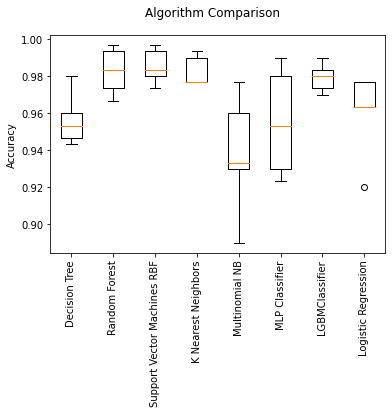
\includegraphics[width=\linewidth]{./figures/results_model_comparison_preprocessed_full_data_lab.png}
			    \caption{Preprocessed full data}
			  \end{subfigure}
			  \caption{Model selection for lab data}
			  \label{fig5.6}
			\end{figure} 
			
			After passing through the model selection phase, we tuned two models Random Forest and support vector machines, to classify the preprocessed datasets. 
			As explained in the methodology section, we used six different metrics to evaluate the performance of the UJI Indoor dataset. 
			In figure~\ref{fig5.7}, we can visualize the performance of these two models again the six predefined metrics for the complete Uji Indoor dataset and each building dataset individually. 
			We see that Random Forest tends to perform generally better than the support vector machines for all the metrics. 
			
			The performance of Random Forest for all four datasets is comparable in terms of accuracy, precision, recall, and F1 score. 
			However, we can see that mean squared error loss for Random Forest amongst the datasets vary where the loss is maximum for building 1 and least for building 0. 
			This phenomenon is fascinating as the accuracy is inverse to MSE; it is best for building 1 and worst for building 0. 
			This development can be explained since the area of building 0 is significantly less than building 1; hence when a prediction gets wrong in building 1, it generally is at a greater distance. 
			
			We also used recall metrics in-depth to analyze the performance of these two models. 
			The comparison analysis by recall quartiles reveals a total of 549 rooms fall within the high recall range of 80-100\% in the entire dataset, whereas 551 rooms fall within the high recall range of 80-100\% when adding up individual building algorithms. 
			The performance here is also comparable, so we selected all the whole dataset and individual building datasets. 
			
			\begin{figure}[!htb]
			  \centering
			  \begin{subfigure}[b]{0.48\linewidth}
			    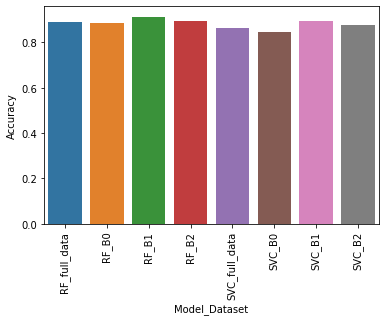
\includegraphics[width=\linewidth]{./figures/Accuracyfinal_results.png}
			     \caption{Accuracy}
			  \end{subfigure}
			  \begin{subfigure}[b]{0.48\linewidth}
			    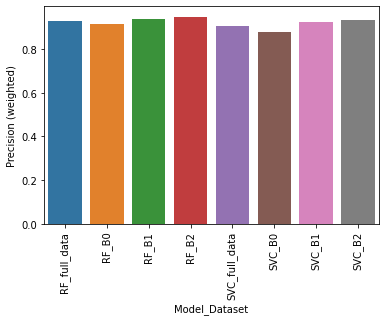
\includegraphics[width=\linewidth]{./figures/Precision (weighted)final_results.png}
			    \caption{Precision}
			  \end{subfigure}
			  \begin{subfigure}[b]{0.48\linewidth}
			    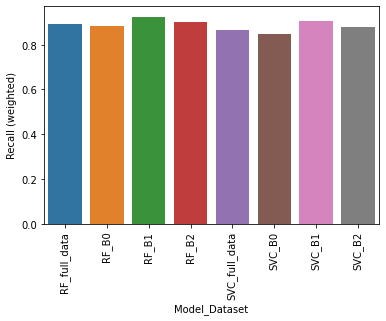
\includegraphics[width=\linewidth]{./figures/Recall (weighted)final_results.png}
			    \caption{Recall}
			  \end{subfigure}
			  \begin{subfigure}[b]{0.48\linewidth}
			    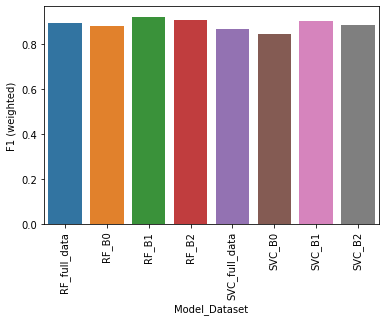
\includegraphics[width=\linewidth]{./figures/F1 (weighted)final_results.png}
			    \caption{F1 Score}
			  \end{subfigure}
			  \begin{subfigure}[b]{0.48\linewidth}
			    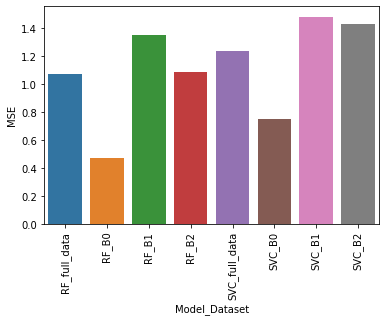
\includegraphics[width=\linewidth]{./figures/MSEfinal_results.png}
			    \caption{MSE}
			  \end{subfigure}
			  \begin{subfigure}[b]{0.48\linewidth}
			    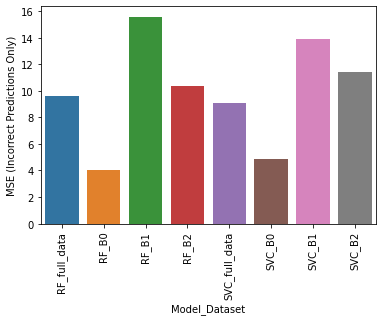
\includegraphics[width=\linewidth]{./figures/MSE (Incorrect Predictions Only)final_results.png}
			    \caption{MSE (Incorrect Predictions Only}
			  \end{subfigure}
			  \caption{Model Assessment for Ujiindoor dataset}
			  \label{fig5.7}
			\end{figure} 
			
			Similarly, we also passed Random Forest and Support Vector Machine through hyperparameter tuning process for the BLE and Lab dataset. 
			In figure~\ref{fig5.8}, we can see the performance of these tuned models. 
			We see that the performance gets better for all metrics as compared to untuned models. 
			However, still, we can see that the BLE model performs worse as compared to Lab dataset. 
			The low performance also points to the reason that there are 1420 observations for 135 locations in the BLE dataset, whereas 4 locations in the Lab dataset consist of 1500 user readings. 
			The enrichment of the dataset significantly improves the performance of the localization process. 
			
			
			\begin{figure}[!htb]
			  \centering
			  \begin{subfigure}[b]{0.48\linewidth}
			    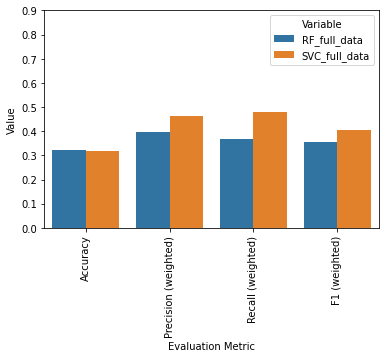
\includegraphics[width=\linewidth]{./figures/final_results_comparison_ble.png}
			     \caption{BLE data}
			  \end{subfigure}
			  \begin{subfigure}[b]{0.48\linewidth}
			    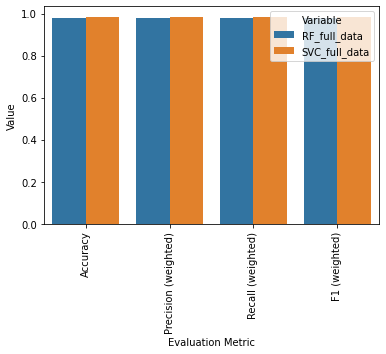
\includegraphics[width=\linewidth]{./figures/final_results_comparison_lab.png}
			    \caption{Lab data}
			  \end{subfigure}
			  \caption{Model Assessment for other datasets}
			  \label{fig5.8}
			\end{figure}
			
			
			Finally, we evaluated the performance of the Principal Component Analysis of our full primary dataset. 
			We can visualize the strength of this dimension reduction technique in figure~\ref{fig5.9}. 
			We assessed the performance at 20\%, 40\%, 60\%, 80\%, and 100\% of the dataset.  
			We visualize the performance trend of the random model in terms of accuracy as the size of the dataset increases.
			Fascinatingly there is not much variation in the performance, which seems to be saturated at around 40\% dataset mark. This evaluation is practical when we would preprocess the dataset for the regression problem. 
			
			
			\begin{figure}[!htb]
				\centering
				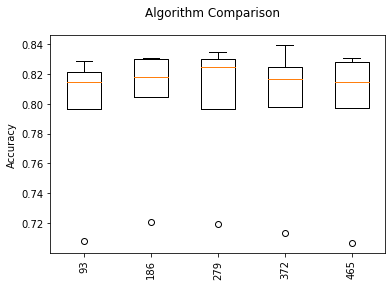
\includegraphics[width=0.8\linewidth]{./figures/pca_results200.png}
				\caption{Performance Comparison using PCA}
				 \label{fig5.9}
			\end{figure} 
			
			The researchers at the School of Computer Science and Engineering Nanyang Technological University, Singapore benchmarked 86.34\% on the UJI Indoor dataset, whereas our experiments have achieved an accuracy of 88.82\%,
			We have selected the random former as the most optimal classifier in our experimentation for further cascaded model analysis.

\newpage
\FloatBarrier
		\section{Modelling as a Regression Problem}

			We analyzed our full dataset using the multi-variable multi-variate regression analysis. 
			We analyzed principal component analysis (PCA) effectiveness on our dataset and selected the first 150 dimensions to perform our regression analysis. 
			We used xy-coordinates based on latitude and longitude as labels and deployed the model selection process on our transformed dataset. 
			Using nested cross-validation, we trained eight different multi-variate regressors and assessed their performance based on root mean squared (RMSE) value. 
			In figure~\ref{fig5.10}, we can visualize the performance of various models on our dataset. Among all the variants, K-Nearest Neighbour and Random Forest perform the best. 
			We can also see that there is not much variation among the cross-validation folds. Hence, we select KNN as our global regressor.
			
			\begin{figure}[!htb]
				\centering
				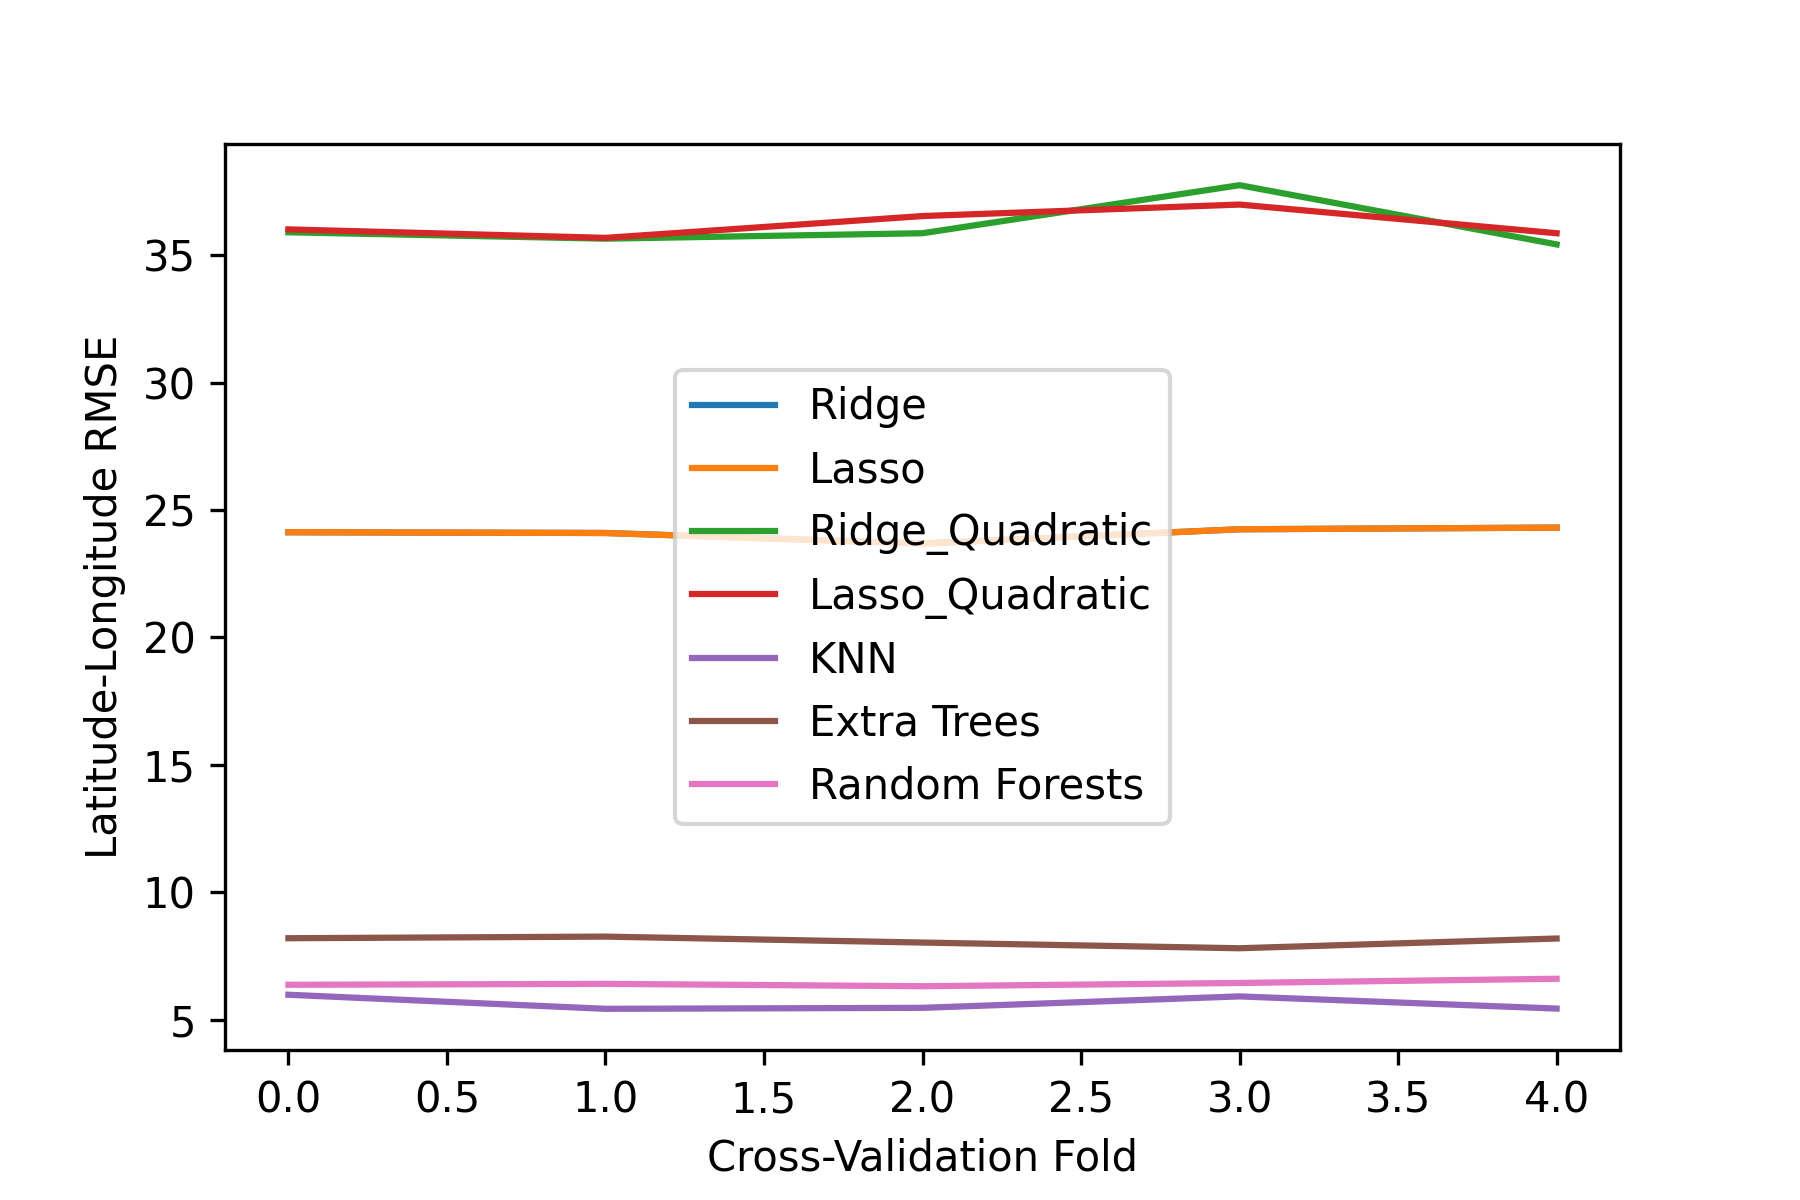
\includegraphics[width=0.8\linewidth]{./figures/nested_crossval_results.png}
				\caption{Nested cross validation results for regression}
				 \label{fig5.10}
			\end{figure}
			
			We passed KNN through the model tuning phase after its selection in the previous phase. 
			The performance of the model improves after its optimal hyperparameters are defined. 
			We also analyzed the performance of the model on per building per floor regression. 
			As depicted in figure~\ref{fig5.11}, the model's performance on a per-floor basis is better than the overall dataset. 
			Among the three buildings, the performance is Building 0, which could be correlated to the fact that its size is the smallest among the three buildings, and its structure is relatively compact. 
			
			We also detected a specific anomaly on floor 4 of Building 2, showing the maximum loss on training and validation datasets.
			This detection refers to the fact that the number of observations on this floor is pretty low as compared to other floors of this building, and the size of this building is more significant than Building 0, which in turn emphasizes the importance of the number of readings and the optimization of user locations while taking the observations.  
			
			
			\begin{figure}[!htb]
				\centering
				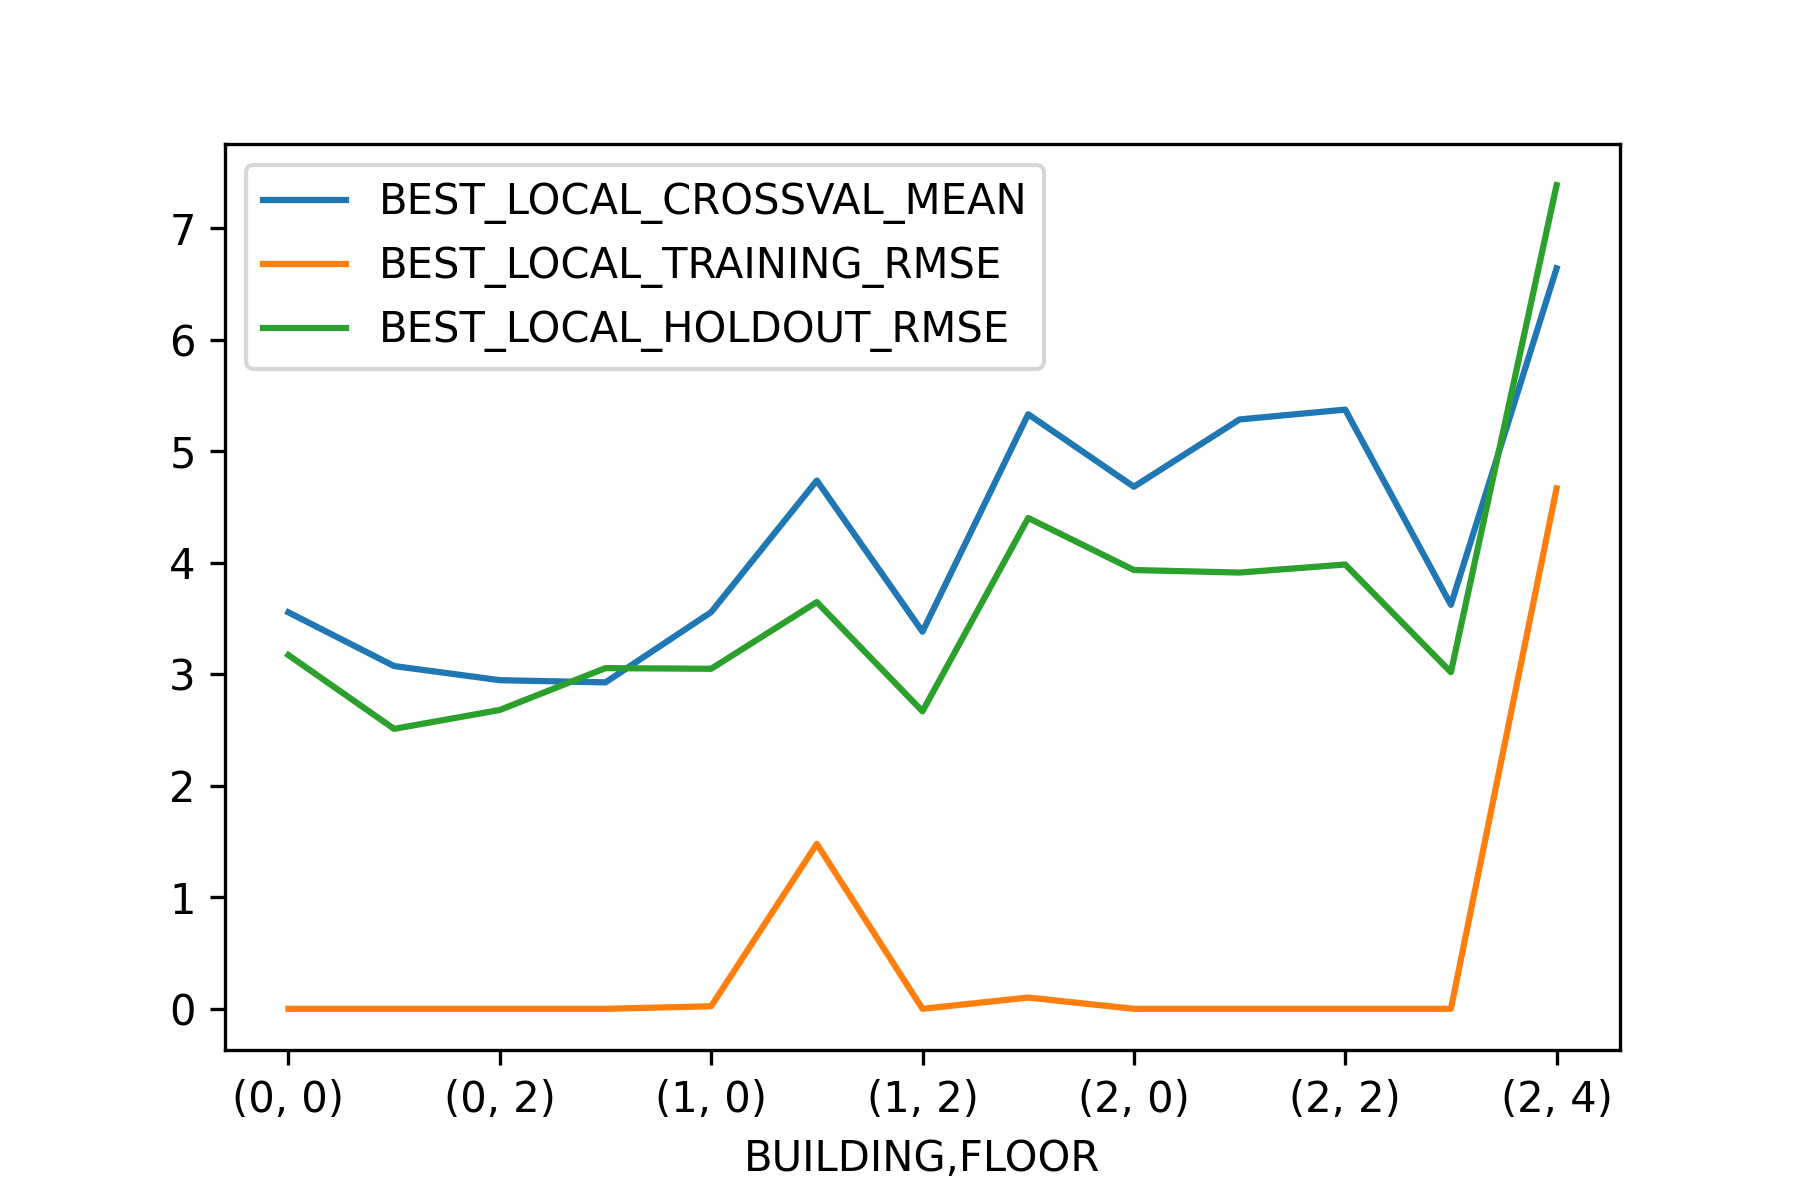
\includegraphics[width=0.8\linewidth]{./figures/best_local_metric_df.png}
				\caption{Performance evaluation of per building per floor regression models}
				 \label{fig5.11}
			\end{figure}
			
			We have selected the K-Nearest Neighbour as the most optimal regressor in our experimentation for further analysis.

		\section{Modelling as a Multi Cascaded Classification and Regression Problem}

			We developed an integrated three-stage multi cascaded machine learning model for predicting user location in our primary dataset. 
			We predicted the user's building with a tuned Random Forest model on the full dataset in the first stage. 
			As depicted in figure~\ref{fig5.12}, the performance of our model is nearly perfect as the dataset is of outstanding quality concerning buildings.
			
			
			
			
			\begin{figure}[!htb]
				\centering
				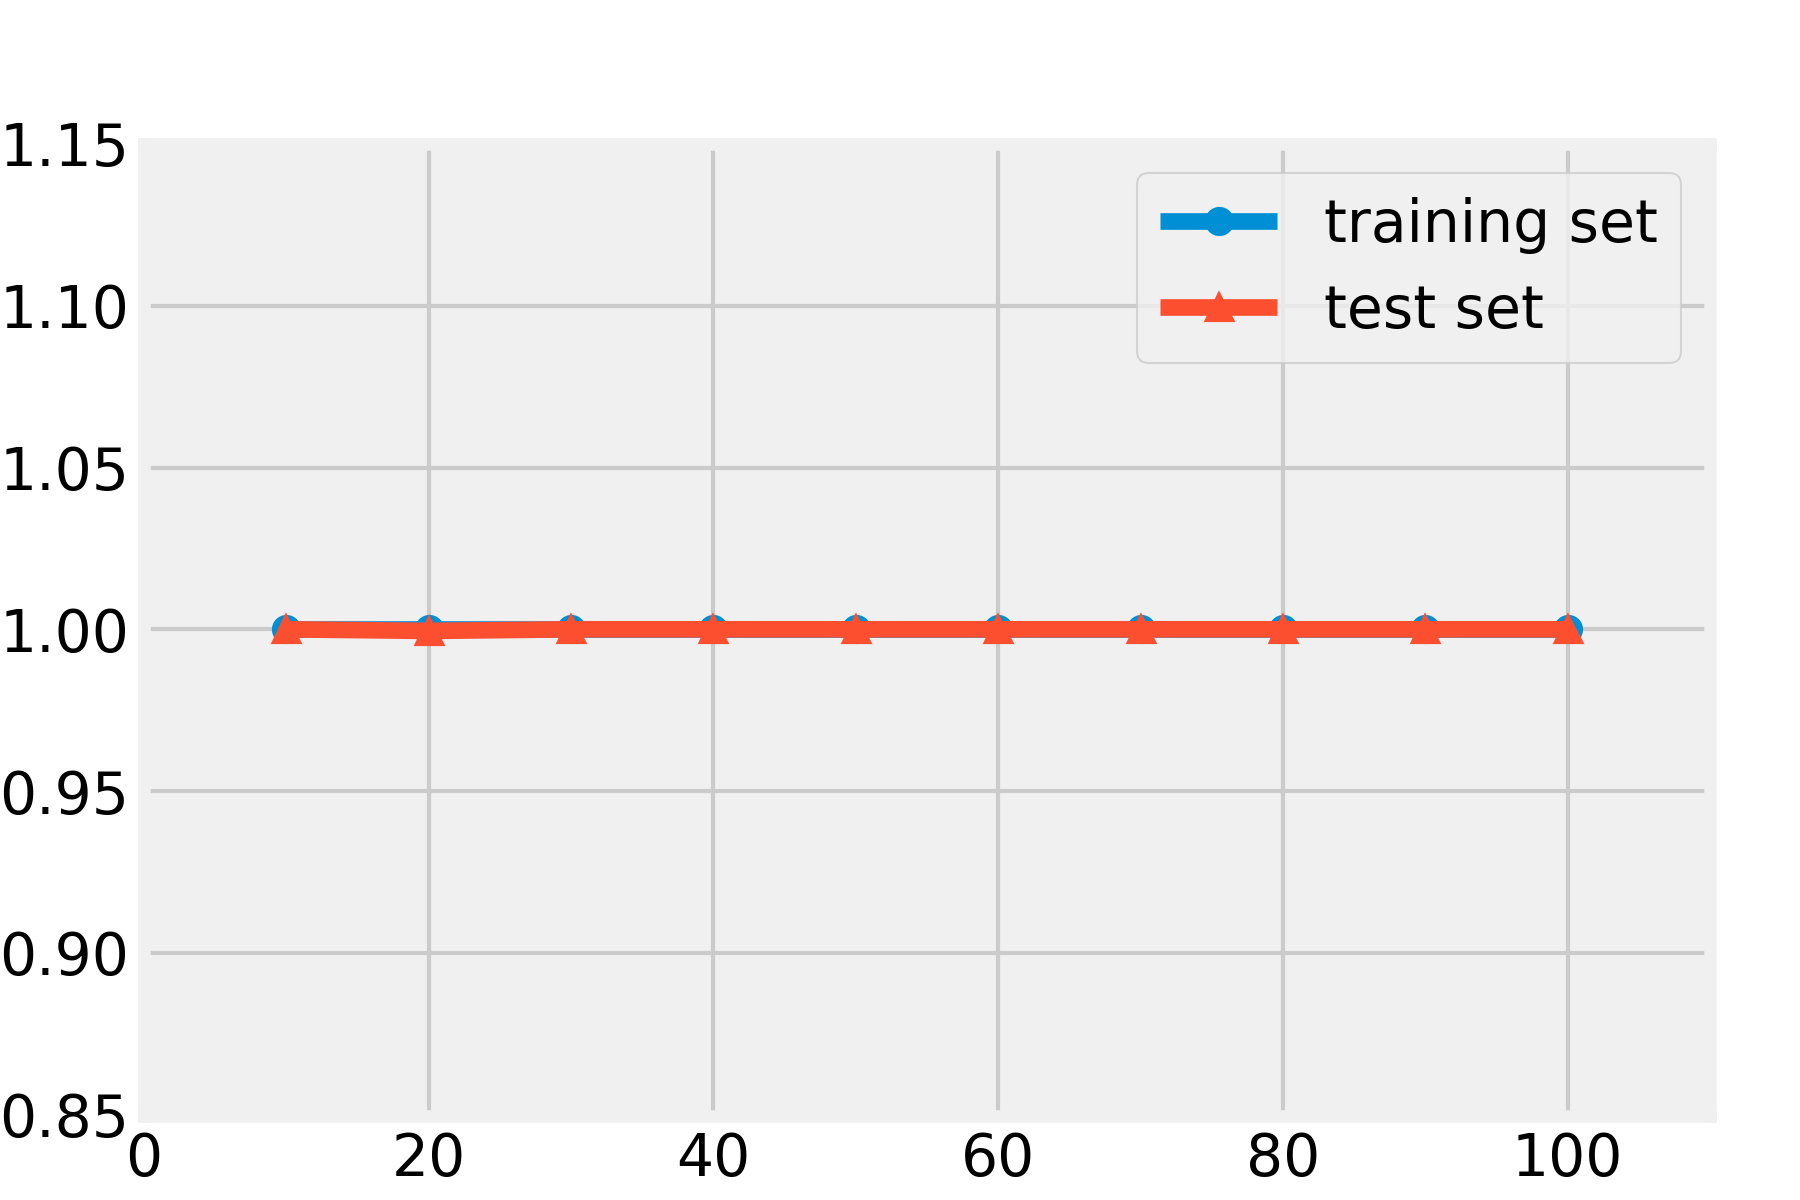
\includegraphics[width=0.8\linewidth]{./figures/plot_learning_curves_building_classification.png}
				\caption{Performance evaluation of  building classifier}
				 \label{fig5.12}
			\end{figure}
			
			The second stage of the cascaded model involves the prediction of the floor. 
			We took two approaches to predict the floor of the user while taking the reading. 
			Initially, we trained the model to predict the floor without using the information of the predicted building. 
			The results were not so good as we only reached a maximum of 68\% on the test dataset, as elucidated in figure~\ref{fig5.13}.
			
			\begin{figure}[!htb]
				\centering
				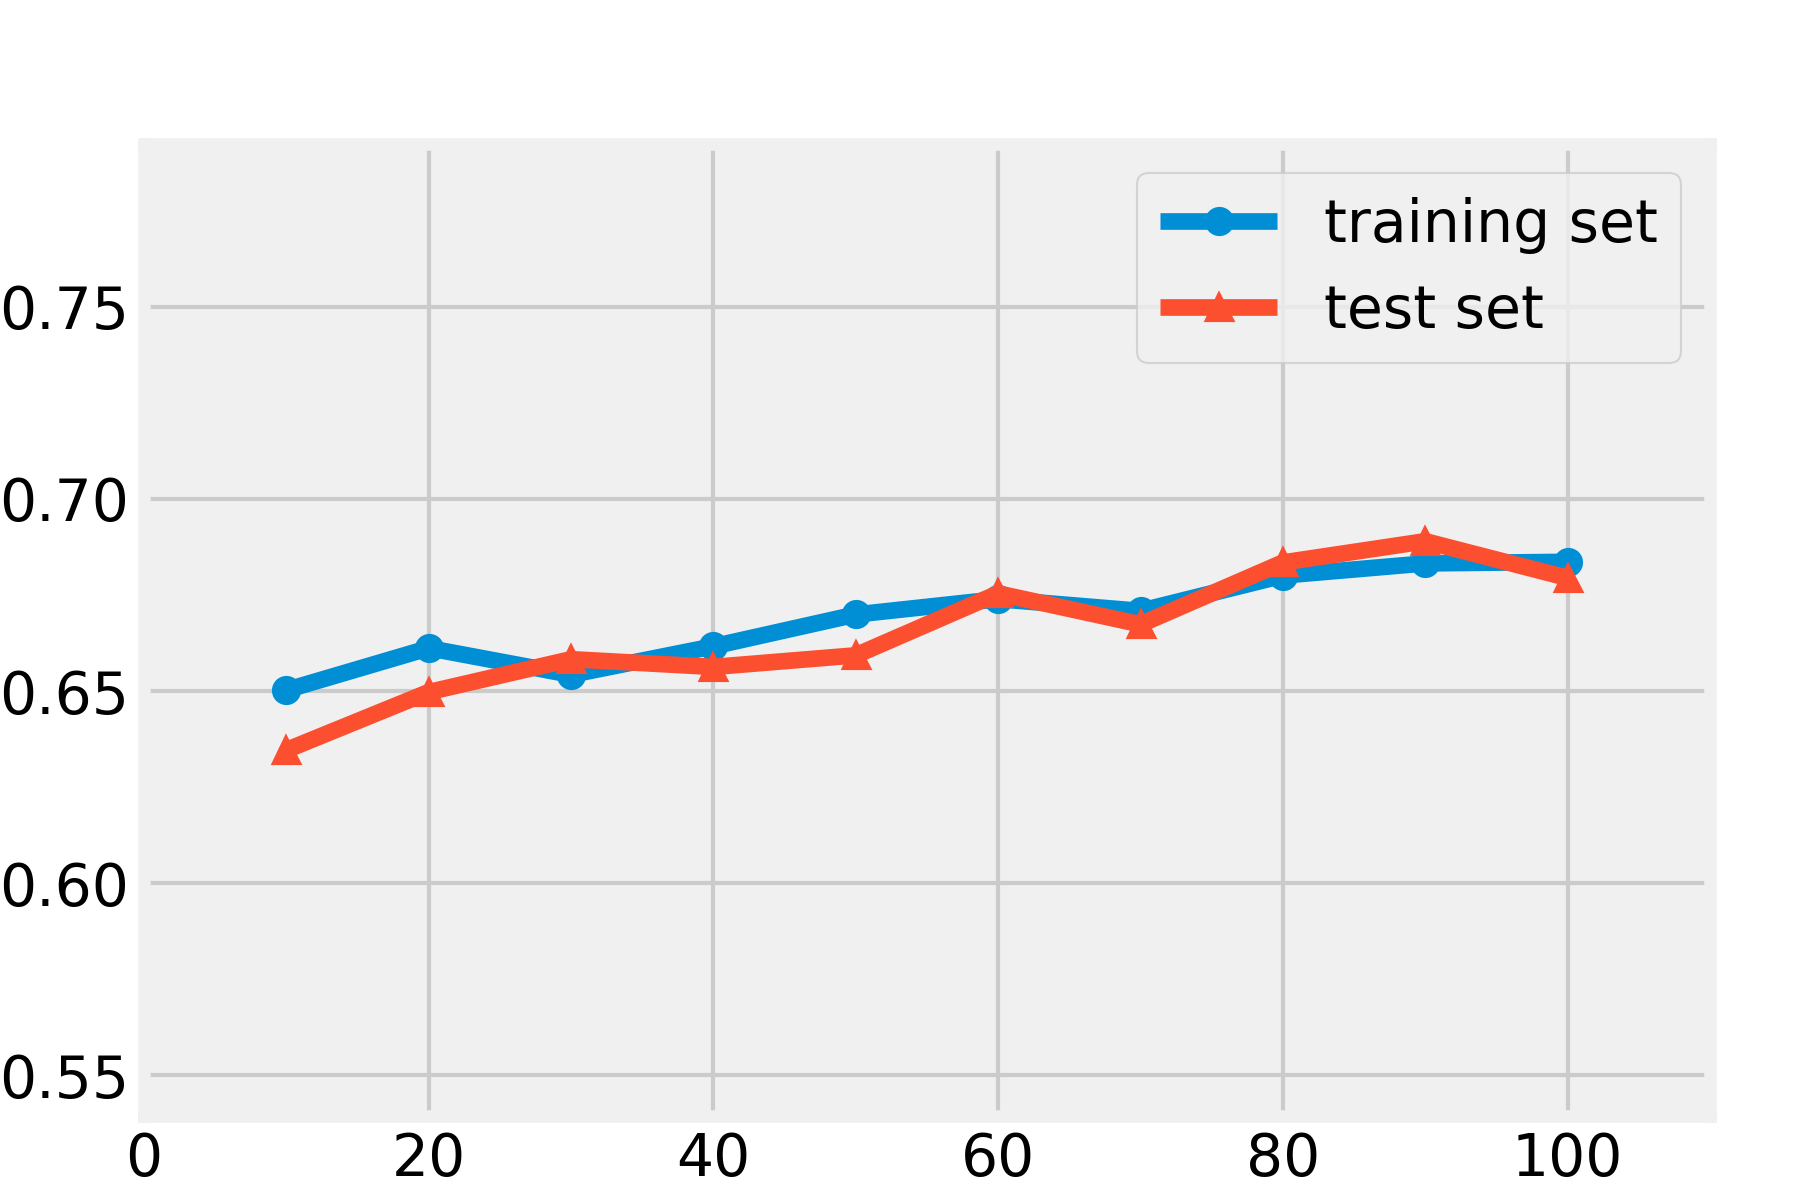
\includegraphics[width=0.8\linewidth]{./figures/plot_learning_curves_global_floor_classification.png}
				\caption{Performance evaluation of global floor classifier}
				 \label{fig5.13}
			\end{figure}
			
			In order to improve the performance of our floor prediction model, we used the information of predicted building from stage one of the cascaded classifiers. 
			As illustrated in figure~\ref{fig5.14}, the performance of the hyperparameter optimized Random Forest model improves significantly on both training and hold out datasets when we use building information in addition to signal strength variables. 
			
			\begin{figure}[!htb]
				\centering
				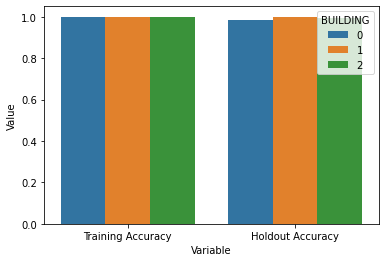
\includegraphics[width=0.8\linewidth]{./figures/best_local_floor.png}
				\caption{Performance of floor per building classification models}
				 \label{fig5.14}
			\end{figure}
			
			
			
			Stage three of the classifier integrates a K-Nearest Neighbour regression model. We trained and analyzed both the global regression model and per floor per building regressor. 
			The performance of the global regressor is notably better than the per floor per building regressor. 
			We used the custom evaluation metric to analyze our overall cascaded model. 
			This metric involves both penalties for floor and building, and the root mean square error of the regressor. 
			The results as shown in figure~\ref{fig5.15}, shows excellent performance of both training and test dataset. 
			Again, the performance of floors with less data is worse than the floors with more data, which emphasizes a need for optimized data acquisition for indoor localization.
			
			\begin{figure}[!htb]
			  \centering
			  \begin{subfigure}[b]{0.48\linewidth}
			    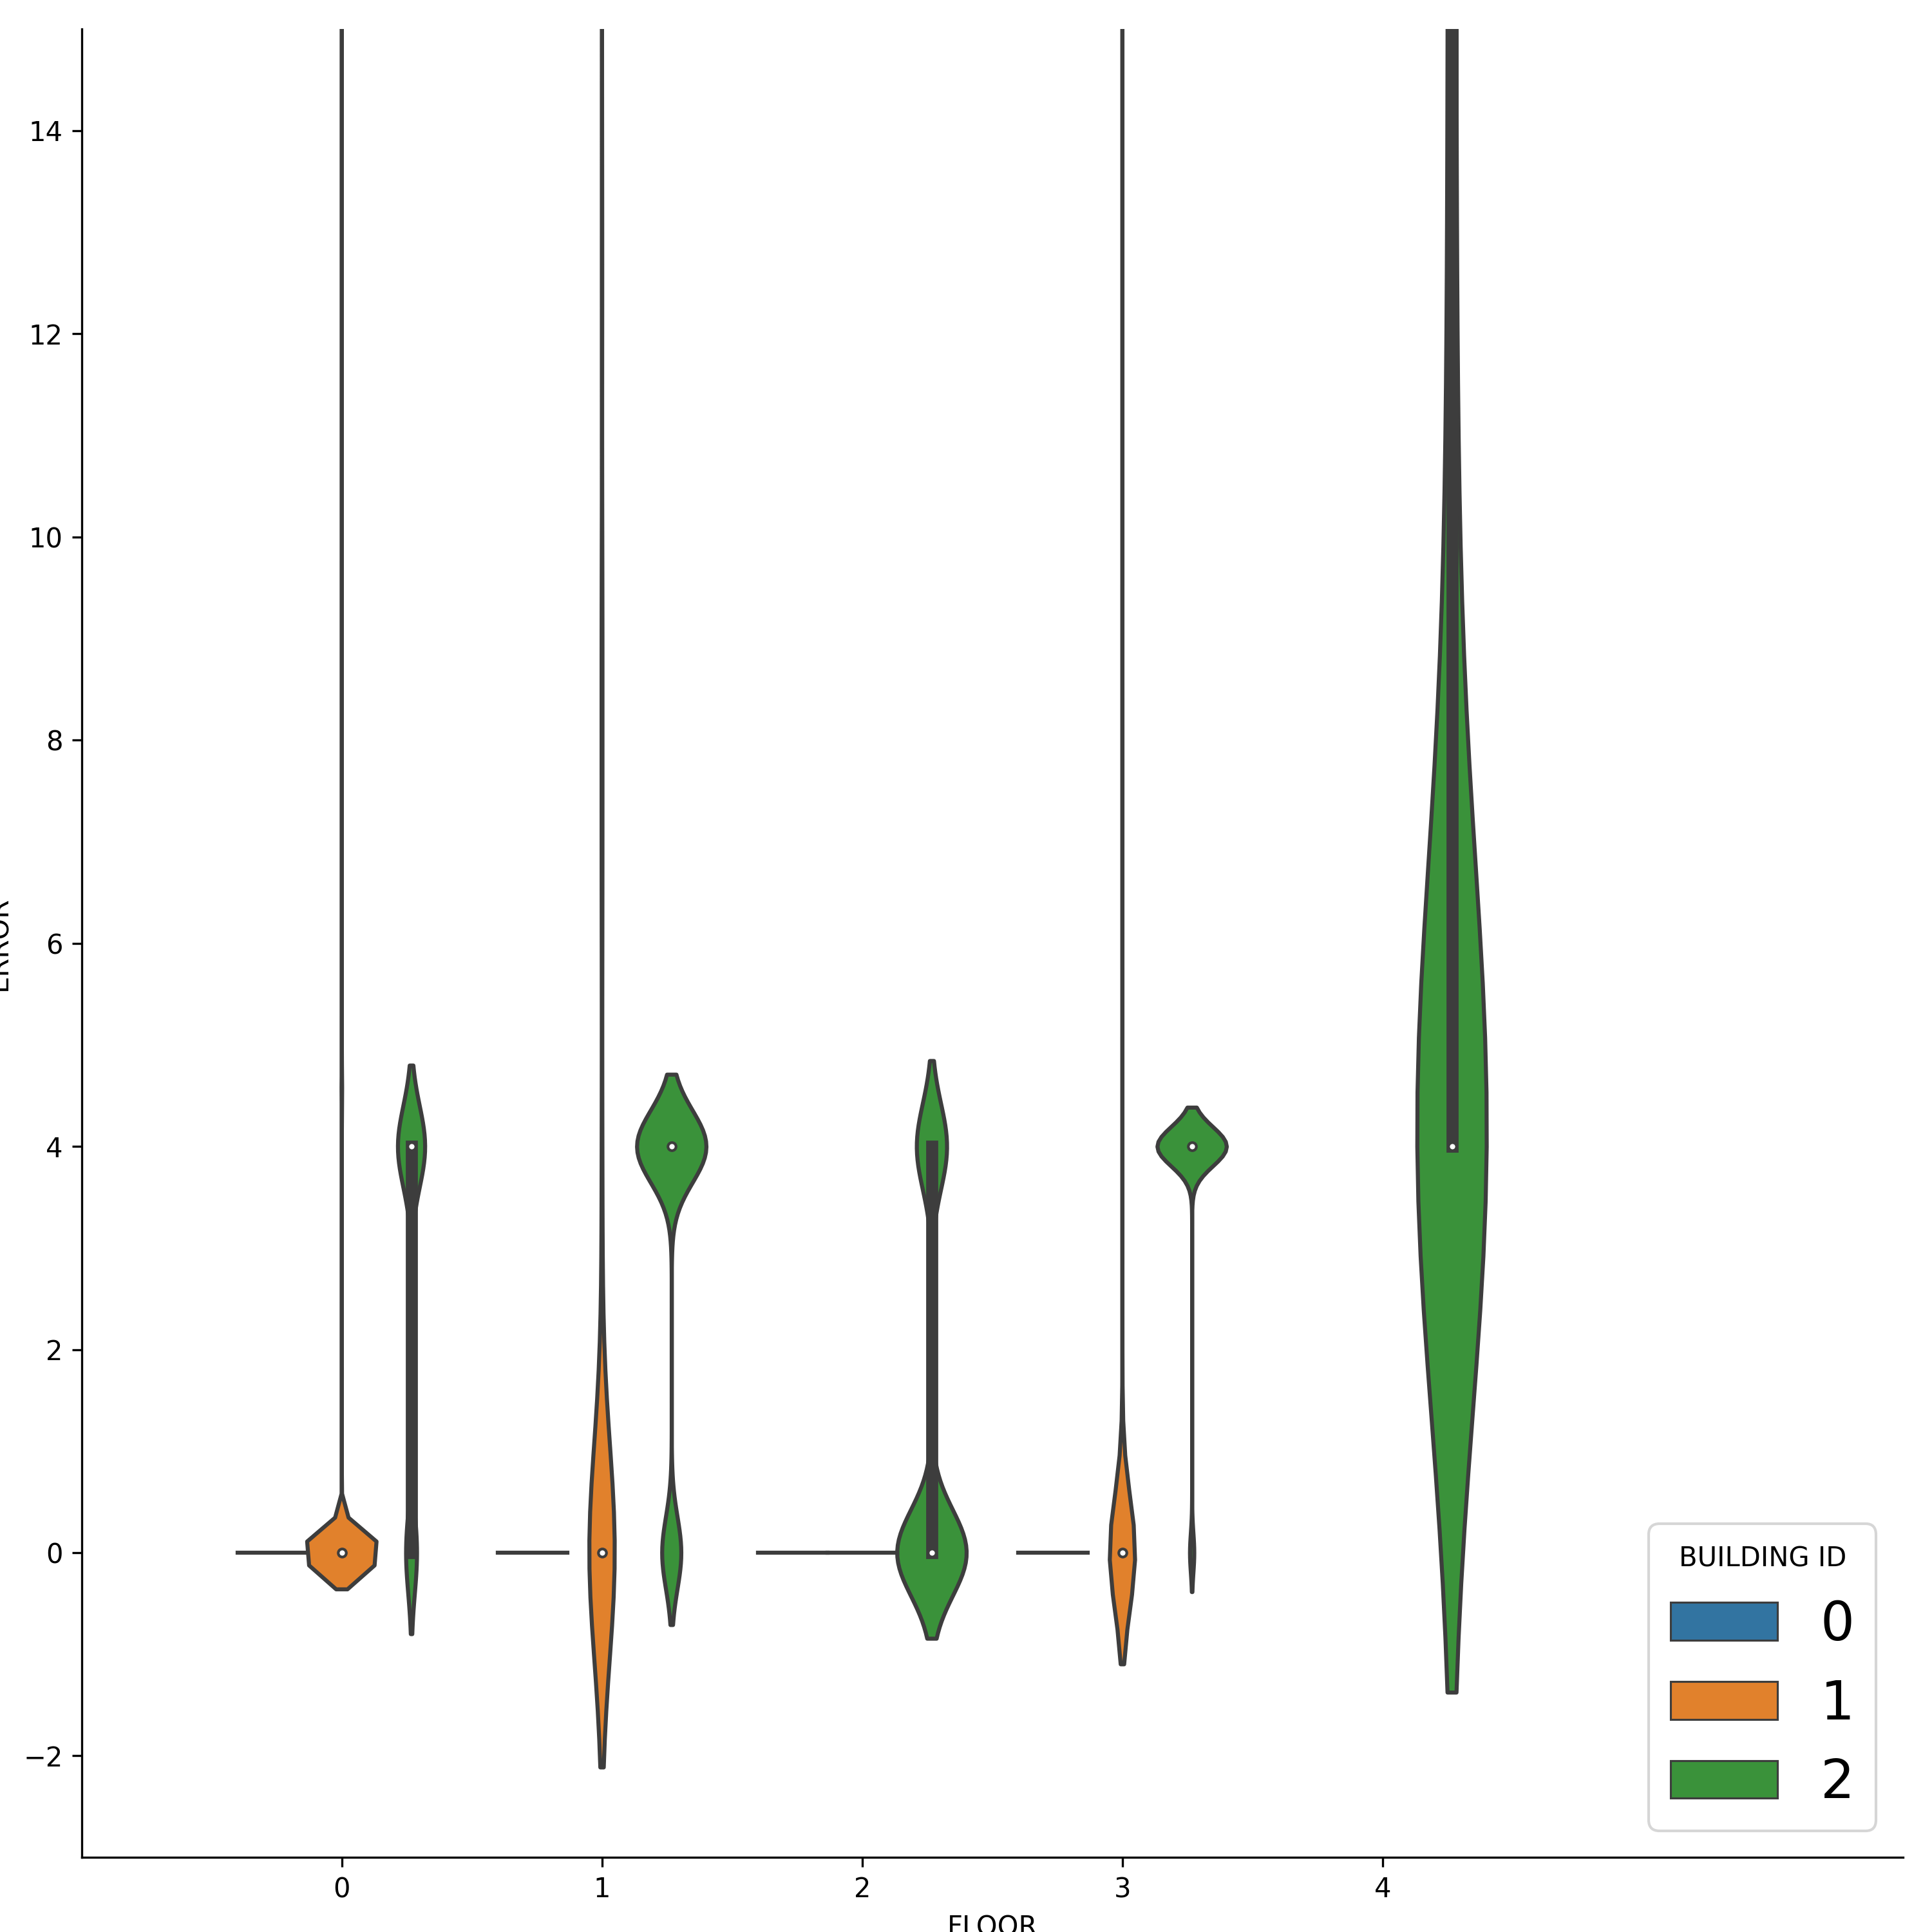
\includegraphics[width=\linewidth]{./figures/penalty_train.png}
			     \caption{Penalty on training dataset}
			  \end{subfigure}
			  \begin{subfigure}[b]{0.48\linewidth}
			    \includegraphics[width=\linewidth]{./figures/penalty_test.png}
			    \caption{Penalty on test dataset}
			  \end{subfigure}
			  \caption{Model Assessment for cascaded models}
			  \label{fig5.15}
			\end{figure}

		\section{Trilateration Methodology for localization of Access Points}

			Trilateration methodology is used to determine the location of all WAPs. 
			Initially, we visualized the location of all the users while taking the observations using their position coordinates. 
			The coordinates given in the UTM scale were converted to latitude and longitude on the GPS scale. 
			In figure~\ref{fig5.16}, we plotted the location of all these users on google maps. 
			It can be seen that the image refers ideally to the three buildings presented in the dataset description.
		
		\begin{figure}[htb!]
			\centering
			\includegraphics[width=1\linewidth]{./figures/google_maps_users.png}
			\caption{Location of users on google maps}
			 \label{fig5.16}
		\end{figure}
		
			After performing the trilateration process, we extracted the coordinates for all the WAPs detected at least once by the user. 
			We did not consider WAPs outside the scope of these buildings, which were not detected even once by any user. 
			This consideration was because our methodology depends upon mean squared error for distances between users and the respective WAP. 
			We can use this methodology to detect the location of WAPs using coordinates but without any information to the floor of the access point. 
			In figure~\ref{fig5.17}, we represented these WAPs on google maps, depicting a uniform distribution of these access points. 
			This information could be utilized to optimize the location of access points in these buildings by detecting the low coverage areas.

		\begin{figure}[!htb]
			\centering
			\includegraphics[width=1\linewidth]{./figures/google_maps_waps.png}
			\caption{Location of WAPs on google maps}
			 \label{fig5.17}
		\end{figure}


	\chapter{Conclusions}
		\section{Final Remarks}

			In this thesis, we have discussed a detailed description of various indoor techniques (RSSI, channel state information, fingerprint analysis, angle of arrival, time of flight, and time difference of arrival) and technologies (as WiFi, Bluetooth, Zigbee, acoustics, optical, and RFID). 
			We also presented several use cases for the application of indoor positioning systems (IPS) to emphasize their importance, especially after the proliferation of intelligent devices.
			
			This thesis presented a thorough application of various machine learning techniques for indoor localization on RSSI-based fingerprinting methodology. 
			We evaluated the problem statement from three different approaches. 
			In the first approach, we developed a grid-based approach to train and evaluate various machine learning classification models with an end-to-end pipeline with feature engineering, model selection, model hyperparameter tuning, and model training. 
			We applied and evaluated our approach with three independent datasets. 
			We evaluated and critically analyzed the results obtained from these different datasets. 
			Moreover, an essential contribution of this thesis is to provide a new state-of-the-art against space labelling on the UJI Indoor dataset. 
			The existing benchmark of 86.34\% on the UJI Indoor dataset was achieved by the researchers at the School of Computer Science and Engineering Nanyang Technological University~\cite{yean2020feature}, Singapore, whereas our experiments have achieved an accuracy of 88.82\% using Random Forest classifier.
			
			Moreover, the second machine learning approach that this thesis applied was to treat indoor localization as a multivariate regression one. 
			We applied dimension reduction techniques and feature engineered our dataset from a logarithmic to a linear scale. 
			We trained and tuned hyperparameters with nested cross-validation of various regression models on the UJI Indoor dataset. 
			Our best trained K-Nearest Neighbour regression model achieved an RMSE error of 3.637 meters.
			
			Furthermore, the third approach we developed in this thesis was cascaded machine learning models. 
			We stacked two classifiers with one's output feeding the other to predict the user's building and floor (per building) location on the UJI Indoor dataset. 
			We stacked a global multivariate regressor to predict the user's location using latitude and longitude coordinates with these two classifiers. 
			We also studied and applied a novel evaluation metric to analyze the results of our cascaded model.
			
			Finally, we developed and discussed the application of trilateration methodology in this thesis. 
			We converted trilateration from a geometrical domain to an optimization one. 
			We applied this optimization approach on our primary dataset to locate the positions of WiFi access points using the RSSI signal strength of users present in its range. 

		\section{Future Work}
			The primary constraint we faced while conducting this study was the availability of good-quality public datasets. 
			There is a void of a proper framework to standardize the data acquisition process. 
			At present, no standard is governing the process of data acquisition in indoor localization. 
			There should be a development of a proper framework for this process to scale its usability. 
			While developing the framework, we would also have to consider the aspect of GDPR, data privacy, and governance.
			
			Standardizing datasets would provide the artificial intelligence scientist community with good quality publicly available resources for further research into the domain. 
			Along with the machine learning techniques used in this thesis, the novel techniques of deep neural networks and natural language processing can also be applied and studied on indoor positioning systems to develop state-of-the-art benchmarking of results.   
			
			One main trade-off that we studied and analyzed in this thesis is grid intensity and discreteness of the results while treating indoor localization as a grid-based fingerprinting problem. 
			As evaluated in the case of the BLE dataset, the accuracy was low due to the high intensity of the grids.
			This problem could be an area of research that needs further attention to optimize the compensation between accuracy and resolution of the indoor positioning systems. 
			
			Finally, one of the research-area this thesis leads to is optimizing area coverage of the WiFi access points. 
			The planning and installation of WiFi access points in complex multi-building infrastructures could be aided with the help of the trilateration methodology studied in this thesis. 
			In the field of ICT, the impact of trilateration methodology and machine learning techniques in optimizing various signal propagation technologies like WiFi, Bluetooth, RFIDs, etc., needs further research.  


	\appendix
	
	\printbibliography[heading=bibintoc] % biblatex

	
	\acknowledgements
		First and foremost, I would like to thank the Almighty Allah, the author of knowledge and wisdom, for His countless blessings. 
		Furthermore, I desire to pay my regards to my parents-Mr. and Mrs. Mohammad Razzaq for their unconditional love and prayers.
  
		I wish to extend my sincere gratitude to the complete faculty of Masters in Artificial Intelligence at the University of Bologna for their assistance. 
		I would like to express my indebtedness to my thesis supervisor Dr. Claudio Sartori for his guidance and continuous encouragement. 
		Without his enlightened counselling and persistent help, this dissertation would not have been possible.
		
		I owe a deep sense of gratitude to Dr. Luca Salvatore Lorello for his keen interest in my progress at every stage of my thesis. 
		His prompt inspiration, timely suggestions with kindness, and sincere support have enabled me to complete my thesis. 
		I wish to appreciate my classmates Dr. Nicolaas Ruberg and Dr. Giorgio Tsiotas, for their continuous assistance throughout my studies. 
		
		I am highly obliged to Dr. Rohma Tariq for her proofreading and constant moral motivation. 
		Last but not least, I am grateful to Asad Azhar for equipping me with the necessary hardware requirements.  
		
\end{document}